\documentclass[conference]{IEEEtran}
\IEEEoverridecommandlockouts
\usepackage{makecell}
\usepackage{cite}
\usepackage{amsmath,amssymb,amsfonts}
\usepackage{algorithmic}
\usepackage[table]{xcolor}
\usepackage{graphicx}
\usepackage{booktabs}
\usepackage{tikz}
\usepackage{textcomp}
\usepackage{hyperref}
\usepackage{xcolor}
\usepackage{tabularx}  % add this in the preamble
\usepackage{makecell}
\def\BibTeX{{\rm B\kern-.05em{\sc i\kern-.025em b}\kern-.08em
    T\kern-.1667em\lower.7ex\hbox{E}\kern-.125emX}}

\newcommand{\Mypm}{\mathbin{\tikz [x=1.4ex,y=1.4ex,line width=.1ex] \draw (0.0,0) -- (1.0,0) (0.5,0.08) -- (0.5,0.92) (0.0,0.5) -- (1.0,0.5);}}%

\definecolor{phase1color}{rgb}{0.92, 0.93, 1.0}  % Very Light Blue
\definecolor{phase2color}{rgb}{0.90, 1.0, 0.90}  % Very Light Green
\definecolor{phase3color}{rgb}{1.0, 1.0, 0.83}  % Very Light Yellow
\definecolor{phase4color}{rgb}{1.0, 0.90, 0.93}  % Very Light Orange
\definecolor{phase5color}{rgb}{1.0, 1.0, 0.95}  % Very Light Pink


\begin{document}

% \title{\huge MINDER: Machine Learning Framework for Depression Score Analysis in Mindfulness Interventions across Medically Complex Patients}

\title{\LARGE \textbf{MINDER}: \underline{M}achine Learn\underline{I}ng Framework for Depressio\underline{N} Score Analysis in Min\underline{D}fulness Int\underline{ER}ventions across Medically Complex Patients}


\author{\IEEEauthorblockN{1\textsuperscript{st} Nikhileswara Rao Sulake \textsuperscript{†}}
\IEEEauthorblockA{\textit{Department of CSE} \\
\textit{RGUKT}, Nuzvid, India \\}
\and
\IEEEauthorblockN{2\textsuperscript{nd} Sai Manikanta Eswar Machara}
\IEEEauthorblockA{\textit{Department of CSE} \\
\textit{RGUKT}, Nuzvid, India \\}
\and
\IEEEauthorblockN{3\textsuperscript{rd} Divya Katam}
\IEEEauthorblockA{\textit{Department of ECE} \\
\textit{RGUKT}, Nuzvid, India \\}
\thanks{† serves as the Team Leader.}
\thanks{RGUKT: Rajiv Gandhi University of Knowledge Technologies.}
\thanks{This document serves as the final report submitted from Team \textbf{COSESN} for Track-1 of the \textbf{Data Competition at IEEE EMBS BHI 2025}.}
}

\maketitle

\begin{abstract}
Depression prediction in medically complex populations remains challenging due to heterogeneous treatment responses. We present a comprehensive machine learning framework evaluating 40 models across five methodological phases to predict Beck Depression Inventory-II (BDI-II) scores at 12- and 24-week follow-ups post-mindfulness intervention. Using data from 210 patients with diverse medical comorbidities, Transformer and CatBoost models achieved optimal performance (R² = 0.247 and 0.200, respectively). Disease-stratified analysis reveals profound condition-dependent effects: cancer patients show elevated depression (+2.92 points) yet strongest therapy benefits (4.19-point improvement with high engagement), while renal patients exhibit unexpected protective patterns (-4.23 points). SHAP analysis identifies baseline severity ( $\approx$ 40\%), age ($\approx$ 15\%), and therapy engagement ($\approx$ 12\%) as primary predictors. Disease-specific models achieve exceptional accuracy (R² = 0.81–0.93), establishing condition-stratified frameworks as essential for clinical deployment in precision psychiatry. We further implemented rigorous statistical validation using 10,000-iteration bootstrap confidence intervals and Mann-Whitney U tests with effect sizes to address small sample concerns. We performed detailed phase-level and model-level visualizations (radar plots, heatmaps), quantified computational efficiency and hardware requirements, and provided translational guidance for clinical deployment. Code, figures, and reproducibility materials are available at: \href{https://github.com/Nikhil-Rao20/IEEE-EMBS-BHI-25-CSOSEN}{https://github.com/Nikhil-Rao20/IEEE-EMBS-BHI-25-CSOSEN}.
\end{abstract}

\begin{IEEEkeywords}
Depression prediction, machine learning, BDI-II, mindfulness intervention, time-series modeling, ensemble methods, disease-specific analysis, SHAP interpretability
\end{IEEEkeywords}

\section{Introduction}

Depression is one of the most prevalent mental health disorders worldwide. According to the World Health Organization, depression affected an estimated 280 million people worldwide in 2019, equivalent to approximately 5\% of all adults globally, and is a leading cause of disability~\cite{WHO_Depression}. This figure has been updated in more recent analyses; for instance, the 2021 Global Burden of Disease study estimates approximately 332 million people affected~\cite{WHO_DepressionFactSheet}.
To assess depression severity and monitor treatment outcomes systematically, standardized self-report measures have become essential tools in both clinical practice and mental health research.

Among these assessment instruments, the Beck Depression Inventory (BDI) stands as one of the most extensively validated and widely applied tools internationally. Originally developed by Aaron T. Beck in 1961 and subsequently revised as the BDI-II in 1996 to align with DSM-IV diagnostic criteria, this inventory has become a cornerstone in psychiatric and psychological evaluation~\cite{beck1996manual}. The BDI-II comprises 21 items, each rated on a 4-point Likert scale (0--3), yielding a total score ranging from 0 to 63, where higher scores indicate more severe depressive symptoms. Standard cutoff ranges classify individuals into four severity categories: minimal depression (0--13), mild depression (14--19), moderate depression (20--28), and severe depression (29--63)\footnote{A clinically meaningful change is typically defined as a $\geq$5-point reduction or 50\% symptom improvement from baseline, based on established minimal clinically important difference (MCID) thresholds.}. This scoring system makes the BDI-II useful both for initial screening and for tracking treatment progress over time.


Importantly, the BDI-II captures a comprehensive spectrum of depressive symptoms across multiple domains: cognitive symptoms (negative thoughts, difficulty concentrating, feelings of worthlessness), affective symptoms (sadness, loss of pleasure, guilt), and somatic symptoms (changes in sleep, appetite, energy levels, physical discomfort). This multidimensional assessment has proven valuable not only for overall depression severity but also for studying specific symptom clusters, such as anhedonia (loss of interest or pleasure in activities)~\cite{pizzagalli2005reduced, treadway2009worth}. Extensive reliability and validity studies conducted across diverse populations consistently demonstrate strong psychometric performance. The BDI-II exhibits high internal consistency (Cronbach's $\alpha \geq 0.84$) and demonstrates sensitivity to symptom changes during treatment interventions~\cite{beck1996manual}. Its robust measurement properties have enabled successful cross-cultural validations across multiple continents, including adaptations and validation studies in European, Asian, and Latin American populations~\cite{wang2013psychometric, b4}.


In clinical and research practice, the BDI-II is administered across a wide range of settings, from hospitals and outpatient mental health clinics to community health centers and large-scale epidemiological studies. Longitudinal follow-up assessments at fixed intervals—such as 12 weeks (end of intervention) and 24 weeks (follow-up assessment)—enable researchers and clinicians to capture temporal changes in depression severity and evaluate the effectiveness of various interventions. This is particularly valuable for assessing the impact of evidence-based psychological therapies, such as mindfulness-based stress reduction (MBSR) and mindfulness-based cognitive therapy (MBCT), which have shown promise in treating depression, especially in populations with comorbid medical conditions~\cite{hunot2013mindfulness, b5}.


\subsection{The Challenge of Depression in Medically Complex Populations}

Mindfulness-based interventions have shown efficacy in alleviating depressive symptoms among general populations, yet a substantial knowledge gap persists regarding outcome variations across medical comorbidity profiles, particularly in patients with serious conditions such as cancer, cardiovascular disease, renal insufficiency, and physical disabilities, where depression prevalence is heightened by disease burden, functional impairments, pain, and psychological distress from diagnosis and treatment. The interplay among specific medical diagnoses, patient demographics, baseline symptom severity, treatment engagement, and long-term depression trajectories remains underexplored, complicating clinical decisions on tailoring intervention intensity, identifying differentially responsive subgroups, pinpointing non-responders requiring alternative strategies, and determining key predictors of sustained remission. Conventional statistical methods often fail to model the nonlinear, multifaceted interactions in heterogeneous cohorts, whereas machine learning approaches enable robust detection of subtle patterns in high-dimensional data and precise individual-level prognostic predictions.

\subsection{Research Objective}
This study addresses the imperative for personalized prediction of depression outcomes in medically complex populations via a multifaceted machine learning framework. Our objectives encompass: (1) developing and evaluating predictive models for Beck Depression Inventory-II (BDI-II) scores at short-term (12-week) and long-term (24-week) follow-ups, benchmarking diverse architectures for accuracy; (2) quantifying the relative contributions of demographic (age, sex), clinical (baseline severity, comorbidities), and engagement (completion rates, attendance) factors to outcome variance; (3) elucidating temporal shifts in predictor influence across timepoints to discern evolving intervention dynamics; (4) performing condition-specific analyses among cancer, acute coronary syndrome, renal insufficiency, and lower-limb amputation cohorts to delineate heterogeneous treatment responses; and (5) leveraging explainable AI methodologies to render predictions interpretable and clinically viable for decision support.




\section{Dataset and Problem Formulation}

\subsection{Dataset Overview}


We analyzed data from 210 patients from 3 different hospital centers, enrolled in a mindfulness-based intervention for depression, with assessments at baseline, 12-week post-intervention, and 24-week follow-up, enabling evaluation of both short- and long-term outcomes. The dataset was split based on the target features: records with missing targets were assigned to the test set, and the remainder to the training set. Initial preprocessing addressed missing values, duplicates (0\% found), and inconsistencies. This splitting strategy resulted in a balanced distribution of features across training and test sets. For instance, the training set comprised 55.7\% males and 44.3\% females. Medical conditions were similarly represented, with 85\%, 75\%, 52\%, and 83\% of cases included in the training split, respectively. The trend of patient's BDI-II~\footnote{BDI-II severity categories: minimal (0-13) (28\%), mild (14-19) (35\%), moderate (20-28) (23\%), severe (29-63) (14\%). A clinically meaningful change is typically defined as $\ge$5-point reduction.} scores for different conditions is shown in Figure~\ref{fig:bdi_distri_hospital}. Given the competition’s real-world deployment scenario, we adopted a future-prediction split: all records with missing 12-/24-week BDI-II scores (i.e., future patients) were reserved as the test set to simulate prospective clinical use.

\begin{figure*}
    \centering
    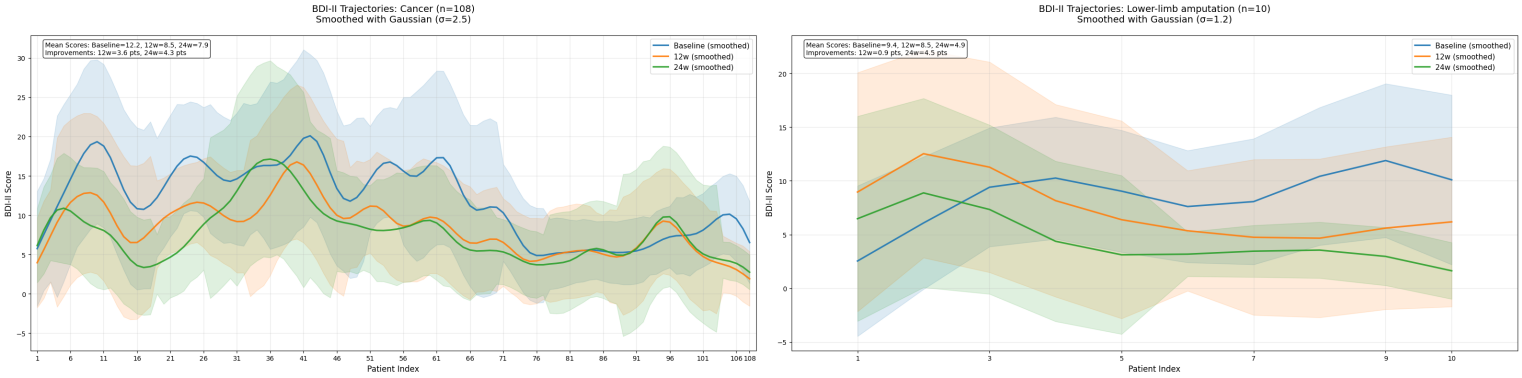
\includegraphics[width=0.48\linewidth]{temp1.png}
    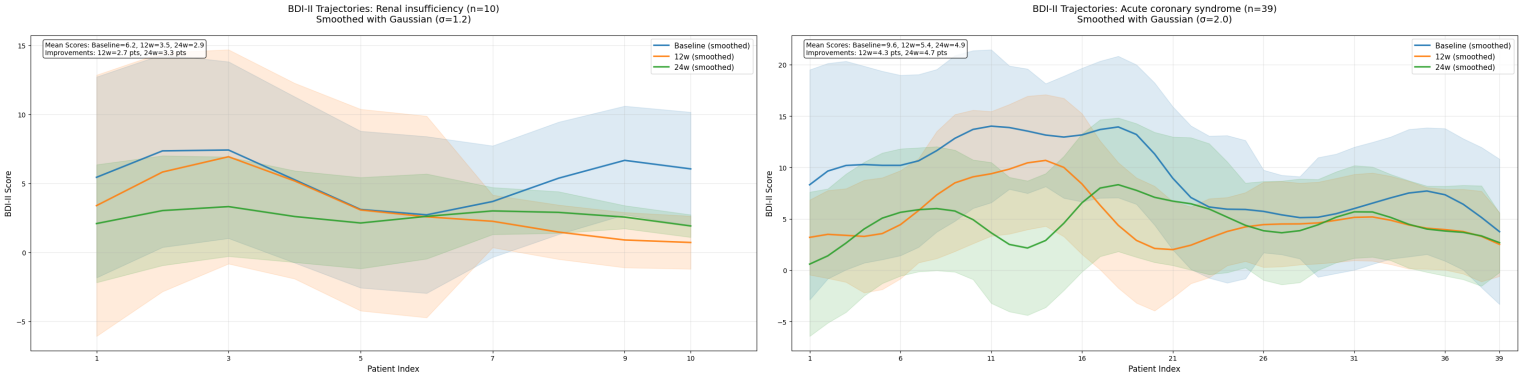
\includegraphics[width=0.48\linewidth]{temp2.png}
    \caption{Comparison of BDI-II scores at baseline, 12-week, and 24-week follow-up, visualizing the score trends for all types of conditions (Cancer, Lower-Limb Amputation, Renal Insufficiency, Acute Coronary Syndrome).}
    \label{fig:bdi_distri_hospital}
\end{figure*}

Four primary medical conditions and seven subtypes were one-hot encoded. BDI-II baseline scores were log-transformed, squared, and categorized for continuous and categorical measures. Age was segmented (young, middle, mature, senior) and scaled nonlinearly via age squared, noting many patients $>45$. Mindfulness engagement was quantified through completion rates and adherence levels (low, medium, high), and sex was binary encoded. Disease burden metrics included total conditions and unique subtypes per patient. Analysis showed patients with lower-limb amputation and renal insufficiency had the highest 12-week success rates (63.9\% and 61.1\%), while cancer and acute coronary syndrome had lower initial rates that declined by 24 weeks. Higher completion improved outcomes for cancer and acute coronary syndrome, but lower completion corresponded to greater improvement for lower-limb amputations.




\begin{table}[ht]
\centering
\caption{Mean BDI-II score improvements from baseline at 12- and 24-week follow-ups across different medical condition types.}
\begin{tabularx}{\linewidth}{|X|c|c|}
\hline
\textbf{Condition Type} & \textbf{12 Week Improvement} & \textbf{24 Week Improvement} \\
\hline
Breast & 4.76 & 5.73 \\ 
Dialysis & 10.00 & 9.00 \\ 
No prosthesis & 0.30 & 4.50 \\ 
Percutaneous CT & 2.25 & 2.125 \\ 
Predialysis & 1.88 & 2.66 \\ 
Prostate & 1.83 & 1.93 \\ 
Revascularization & 4.77 & 5.00 \\ 
\hline
\end{tabularx}
\label{tab:bdii_improvement}
\end{table}


The dataset included 26 numeric features and two targets, with all categorical and clinical variables standardized for machine learning. Features were grouped as: Demographics (age, sex), Clinical Baseline (baseline BDI-II), Medical Comorbidities (Cancer, ACS, Renal, LLA~\footnote{Acute Coronary Syndrome (ACS) and Lower-Limb Amputation (LLA) are abbreviated as shown.} ; see Table~\ref{tab:bdii_improvement} for 12- and 24-week improvements) , Treatment Engagement (session completion, mindfulness; average 71.81\%), and Prediction Targets (BDI-II at 12 and 24 weeks). Patients with higher baseline BDI-II scores showed greater improvements (Table~\ref{tab:severity_metrics_mean}). Patients in the severe category, who received the most intensive engagement, had the highest improvements of 16.2 and 17.8.


\begin{table}
\centering
\caption{Baseline Severity and Improvement Metrics (Mean Values)}
\label{tab:severity_metrics_mean}
\begin{tabularx}{\linewidth}{|X|X|X|X|X|}
\hline
\textbf{Baseline Severity} & \textbf{Completion Rate} & \textbf{12w Improvement} & \textbf{24w Improvement} & \textbf{BDI-II Baseline} \\
\hline
Minimal & 0.721 & 1.239 & 1.632 & 6.639 \\ 
Mild & 0.707 & 6.250 & 8.071 & 16.353 \\ 
Moderate & 0.704 & 10.800 & 11.857 & 23.348 \\ 
Severe& 0.762 & 16.286 & 17.857 & 35.625 \\
\hline
\end{tabularx}
\end{table}

% \begin{figure}
%     \centering
%     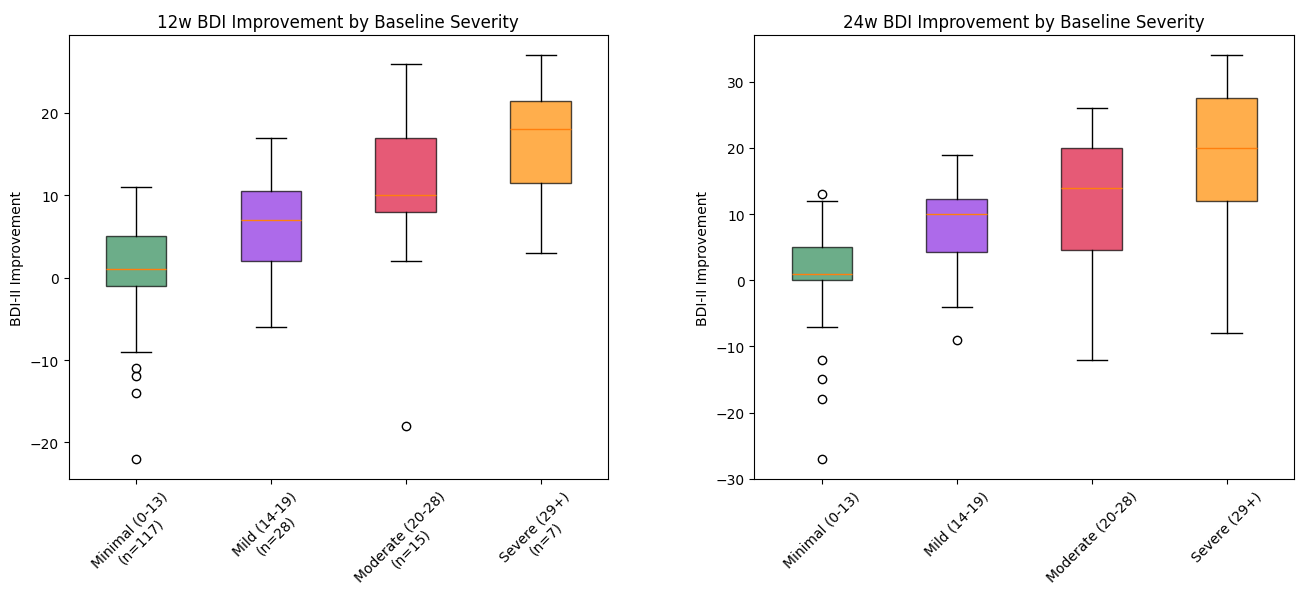
\includegraphics[width=1\linewidth]{bdi_distri_severity.png}
%     \caption{Baseline Severity and Improvement Metrics}
%     \label{tab:severity_metrics_mean}
% \end{figure}



% ----
\section{Planned Methodology}

Our primary objective was to develop robust predictive models to estimate patient's BDI-II scores at 12-week and 24-week follow-ups. To achieve this, we framed the challenge as two independent supervised regression tasks using a rigorous multi-phase models experimentation.
\subsection{Multi-Phase Modeling Strategy}
We implement a systematic five-phase\footnote{Phases indicate increasing model complexity, trained in parallel on identical features. Phase 5 used padding and windowing for variable-length data.} experimental framework designed to comprehensively explore the model complexity spectrum while maintaining interpretability and clinical relevance (Table~\ref{tab:phases}). Linear models provide interpretability and feature importance. Classical ML methods capture non-linear relationships. Ensembles combine multiple perspectives for improved performance. Deep learning explores MLPs, attention, and ResNet-based architectures. Time-series models (LSTM, GRU, Transformer) leverage longitudinal patient data.

\begin{table}[ht]
\centering
\caption{Multi-Phase Modeling Framework}
\label{tab:phases}
\resizebox{\columnwidth}{!}{%
\begin{tabular}{@{}llll@{}}
\toprule
\textbf{Phase} & \textbf{Category} & \textbf{Key Models} & \textbf{\# Models} \\ \midrule
1 & Linear Baselines & Lasso, Ridge, ElasticNet, Bayesian Ridge, etc & 8 \\
2 & Classical ML & Random Forest, SVR variants, KNN, GB, etc & 10 \\
3 & Ensembles & XGBoost, CatBoost, Stacking, Voting, etc & 5 \\
4 & Deep Learning & MLP variants, Attention, ResNet, etc & 7 \\
5 & Time-series & Transformer, LSTM, GRU, Trajectory, etc & 10 \\ \midrule
\multicolumn{3}{l}{\textbf{Total Models Evaluated}} & \textbf{40} \\ \bottomrule
\end{tabular}%
}
\end{table}


\begin{table*}[ht]
\centering
\caption{Model performance metrics at 12- and 24-week follow-ups. The table presents comprehensive results across all five model phases, with the top-performing models highlighted: Top 1 in red, Top 2 in purple, and Top 3 in blue for both 12- and 24-week evaluations. Models within each phase are grouped by cell color, and phases are arranged sequentially from Phase 1 (top-left) to Phase 5 (bottom-right).}
\label{tab:model_performance_phases}
\resizebox{\linewidth}{!}{
\begin{tabular}{@{}lrrrr@{\hspace{0.8em}}|@{\hspace{0.8em}}lrrrr@{}}
\toprule
\textbf{Model} & \textbf{12-Wk $R^2$} & \textbf{12-Wk MAE} & \textbf{24-Wk $R^2$} & \textbf{24-Wk MAE} & \textbf{Model} & \textbf{12-Wk $R^2$} & \textbf{12-Wk MAE} & \textbf{24-Wk $R^2$} & \textbf{24-Wk MAE} \\
\midrule
% Phase 1 (Left) | Phase 3 (Right)
\cellcolor{phase1color}Linear Regression & \cellcolor{phase1color}$-0.03 \pm 0.24$ & \cellcolor{phase1color}$5.18 \pm 0.34$ & \cellcolor{phase1color}$-0.02 \pm 0.25$ & \cellcolor{phase1color}$5.08 \pm 0.65$ & \cellcolor{phase3color}Voting Regressor & \cellcolor{phase3color}$-0.17 \pm 0.35$ & \cellcolor{phase3color}$5.39 \pm 0.55$ & \cellcolor{phase3color}$0.09 \pm 0.30$ & \cellcolor{phase3color}$4.70 \pm 0.42$ \\ \vspace{1pt}
\cellcolor{phase1color}Ridge Regression & \cellcolor{phase1color}$0.15 \pm 0.17$ & \cellcolor{phase1color}$4.79 \pm 0.38$ & \cellcolor{phase1color}$0.09 \pm 0.21$ & \cellcolor{phase1color}$4.73 \pm 0.38$ & \cellcolor{phase3color}Stacking Regressor & \cellcolor{phase3color}$0.07 \pm 0.12$ & \cellcolor{phase3color}$5.18 \pm 0.72$ & \cellcolor{phase3color}$0.11 \pm 0.19$ & \cellcolor{phase3color}$4.80 \pm 0.48$ \\ \vspace{1pt} 
\cellcolor{phase1color}\color{purple}{\textbf{Lasso Regression}} & \cellcolor{phase1color}\color{purple}{\textbf{$0.18 \pm 0.11$}} & \cellcolor{phase1color}\color{purple}{\textbf{$4.71 \pm 0.53$}} & \cellcolor{phase1color}$0.09 \pm 0.18$ & \cellcolor{phase1color}$4.68 \pm 0.43$ & \cellcolor{phase3color}Advanced Stacking & \cellcolor{phase3color}$0.04 \pm 0.16$ & \cellcolor{phase3color}$5.26 \pm 0.66$ & \cellcolor{phase3color}$0.13 \pm 0.18$ & \cellcolor{phase3color}$4.77 \pm 0.46$ \\ \vspace{1pt}
% Phase 1 (Left) | Phase 4 (Right)
\cellcolor{phase1color}\color{blue}{\textbf{Elastic Net}} & \cellcolor{phase1color}\color{blue}{\textbf{$0.16 \pm 0.16$}} & \cellcolor{phase1color}\color{blue}{\textbf{$4.77 \pm 0.43$}} & \cellcolor{phase1color}$0.09 \pm 0.19$ & \cellcolor{phase1color}$4.68 \pm 0.41$ & \cellcolor{phase4color}MLP (Small) & \cellcolor{phase4color}$0.05 \pm 0.09$ & \cellcolor{phase4color}$5.24 \pm 0.65$ & \cellcolor{phase4color}$0.06 \pm 0.14$ & \cellcolor{phase4color}$4.88 \pm 0.08$ \\ \vspace{1pt}
\cellcolor{phase1color}Bayesian Ridge & \cellcolor{phase1color}$0.14 \pm 0.17$ & \cellcolor{phase1color}$4.79 \pm 0.36$ & \cellcolor{phase1color}$0.08 \pm 0.21$ & \cellcolor{phase1color}$4.74 \pm 0.39$ & \cellcolor{phase4color}MLP (Medium) & \cellcolor{phase4color}$0.13 \pm 0.13$ & \cellcolor{phase4color}$4.96 \pm 0.31$ & \cellcolor{phase4color}$0.15 \pm 0.15$ & \cellcolor{phase4color}$4.73 \pm 0.17$ \\ \vspace{1pt}
\cellcolor{phase1color}Huber Regressor & \cellcolor{phase1color}$0.11 \pm 0.16$ & \cellcolor{phase1color}$4.79 \pm 0.49$ & \cellcolor{phase1color}$0.02 \pm 0.20$ & \cellcolor{phase1color}$4.68 \pm 0.21$ & \cellcolor{phase4color}\color{purple}{\textbf{MLP (Large)}} & \cellcolor{phase4color}$-0.04\pm0.18$ & \cellcolor{phase4color}$5.30\pm0.98$ & \cellcolor{phase4color}\color{purple}{\textbf{$0.16\pm0.13$ }}& \cellcolor{phase4color}\color{purple}{\textbf{$4.64\pm0.09$}} \\ \vspace{1pt}
\cellcolor{phase1color}RANSAC Regressor & \cellcolor{phase1color}$-0.37 \pm 0.39$ & \cellcolor{phase1color}$5.98 \pm 1.05$ & \cellcolor{phase1color}$-0.96 \pm 0.76$ & \cellcolor{phase1color}$6.80 \pm 1.49$ & \cellcolor{phase4color}TF MLP (Simple) & \cellcolor{phase4color}$-0.12 \pm 0.16$ & \cellcolor{phase4color}$5.29 \pm 0.85$ & \cellcolor{phase4color}$0.04 \pm 0.06$ & \cellcolor{phase4color}$4.66 \pm 0.12$ \\ \vspace{1pt}
\cellcolor{phase1color}Decision Tree & \cellcolor{phase1color}$-0.07 \pm 0.14$ & \cellcolor{phase1color}$5.19 \pm 0.64$ & \cellcolor{phase1color}$-0.06 \pm 0.40$ & \cellcolor{phase1color}$4.81 \pm 0.63$ & \cellcolor{phase4color}TF MLP (Deep) & \cellcolor{phase4color}$-0.35 \pm 0.70$ & \cellcolor{phase4color}$5.53 \pm 1.27$ & \cellcolor{phase4color}$-0.31 \pm 0.32$ & \cellcolor{phase4color}$5.49 \pm 0.93$ \\ \vspace{1pt}
% Phase 2 (Left) | Phase 4 (Right)
\cellcolor{phase2color}Random Forest & \cellcolor{phase2color}$0.09 \pm 0.19$ & \cellcolor{phase2color}$4.82 \pm 0.45$ & \cellcolor{phase2color}$0.14 \pm 0.25$ & \cellcolor{phase2color}$4.52 \pm 0.44$ & \cellcolor{phase4color}TF ResNet & \cellcolor{phase4color}$0.05 \pm 0.11$ & \cellcolor{phase4color}$4.83 \pm 0.66$ & \cellcolor{phase4color}$-0.31 \pm 0.27$ & \cellcolor{phase4color}$5.31 \pm 0.72$ \\ \vspace{1pt}
\cellcolor{phase2color}Extra Trees & \cellcolor{phase2color}$0.05 \pm 0.25$ & \cellcolor{phase2color}$4.93 \pm 0.36$ & \cellcolor{phase2color}$-0.01 \pm 0.39$ & \cellcolor{phase2color}$4.78 \pm 0.38$ & \cellcolor{phase4color}TF Attention & \cellcolor{phase4color}$0.15 \pm 0.07$ & \cellcolor{phase4color}$4.78 \pm 0.34$ & \cellcolor{phase4color}$0.12 \pm 0.07$ & \cellcolor{phase4color}$4.62 \pm 0.08$ \\ \vspace{1pt}
% Phase 2 (Left) | Phase 5 (Right)
\cellcolor{phase2color}AdaBoost & \cellcolor{phase2color}$0.09 \pm 0.15$ & \cellcolor{phase2color}$4.83 \pm 0.53$ & \cellcolor{phase2color}$0.11 \pm 0.23$ & \cellcolor{phase2color}$4.65 \pm 0.53$ & \cellcolor{phase5color}ARIMA & \cellcolor{phase5color}$-0.21 \pm 0.21$ & \cellcolor{phase5color}$5.71 \pm 0.97$ & \cellcolor{phase5color}$-0.23 \pm 0.25$ & \cellcolor{phase5color}$5.14 \pm 1.27$ \\ \vspace{1pt}
\cellcolor{phase2color}Gradient Boosting & \cellcolor{phase2color}$0.06 \pm 0.19$ & \cellcolor{phase2color}$5.07 \pm 0.48$ & \cellcolor{phase2color}$0.03 \pm 0.26$ & \cellcolor{phase2color}$4.79 \pm 0.54$ & \cellcolor{phase5color}Exponential Smoothing & \cellcolor{phase5color}$-0.20 \pm 0.06$ & \cellcolor{phase5color}$5.87 \pm 0.83$ & \cellcolor{phase5color}$-0.29 \pm 0.38$ & \cellcolor{phase5color}$5.31 \pm 1.53$ \\ \vspace{1pt}
\cellcolor{phase2color}SVR (Linear) & \cellcolor{phase2color}$0.14 \pm 0.12$ & \cellcolor{phase2color}$4.67 \pm 0.58$ & \cellcolor{phase2color}$0.03 \pm 0.15$ & \cellcolor{phase2color}$4.56 \pm 0.26$ & \cellcolor{phase5color}Moving Average & \cellcolor{phase5color}$-0.50 \pm 0.35$ & \cellcolor{phase5color}$6.38 \pm 1.08$ & \cellcolor{phase5color}$-0.40 \pm 0.23$ & \cellcolor{phase5color}$5.80 \pm 1.39$ \\ \vspace{1pt}
\cellcolor{phase2color}SVR (RBF) & \cellcolor{phase2color}$0.15 \pm 0.08$ & \cellcolor{phase2color}$4.73 \pm 0.81$ & \cellcolor{phase2color}$0.11 \pm 0.18$ & \cellcolor{phase2color}$4.49 \pm 0.34$ & \cellcolor{phase5color}LSTM (Simple) & \cellcolor{phase5color}$0.05 \pm 0.06$ & \cellcolor{phase5color}$5.33 \pm 0.48$ & \cellcolor{phase5color}$0.01 \pm 0.03$ & \cellcolor{phase5color}$5.08 \pm 0.34$ \\ \vspace{1pt}
\cellcolor{phase2color}SVR (Poly) & \cellcolor{phase2color}$0.04 \pm 0.22$ & \cellcolor{phase2color}$5.24 \pm 1.06$ & \cellcolor{phase2color}$-0.01 \pm 0.10$ & \cellcolor{phase2color}$4.80 \pm 0.69$ & \cellcolor{phase5color}LSTM (Bi-dir) & \cellcolor{phase5color}$0.13 \pm 0.07$ & \cellcolor{phase5color}$5.13 \pm 0.57$ & \cellcolor{phase5color}$-0.01 \pm 0.03$ & \cellcolor{phase5color}$5.19 \pm 0.34$ \\ \vspace{1pt}
\cellcolor{phase2color}NU SVR & \cellcolor{phase2color}$0.14 \pm 0.07$ & \cellcolor{phase2color}$4.74 \pm 0.91$ & \cellcolor{phase2color}$0.05 \pm 0.10$ & \cellcolor{phase2color}$4.51 \pm 0.56$ & \cellcolor{phase5color}LSTM (Stacked) & \cellcolor{phase5color}$0.13 \pm 0.12$ & \cellcolor{phase5color}$5.03 \pm 0.61$ & \cellcolor{phase5color}$-0.01 \pm 0.01$ & \cellcolor{phase5color}$5.11 \pm 0.37$ \\ \vspace{1pt}
\cellcolor{phase2color}KNN Regressor & \cellcolor{phase2color}$0.13 \pm 0.14$ & \cellcolor{phase2color}$5.01 \pm 0.57$ & \cellcolor{phase2color}$0.12 \pm 0.19$ & \cellcolor{phase2color}$4.55 \pm 0.56$ & \cellcolor{phase5color}GRU & \cellcolor{phase5color}$0.08 \pm 0.05$ & \cellcolor{phase5color}$5.22 \pm 0.47$ & \cellcolor{phase5color}$0.01 \pm 0.04$ & \cellcolor{phase5color}$5.18 \pm 0.37$ \\ \vspace{1pt}
\cellcolor{phase2color}KNN Uniform & \cellcolor{phase2color}$0.15 \pm 0.14$ & \cellcolor{phase2color}$4.95 \pm 0.64$ & \cellcolor{phase2color}$0.01 \pm 0.22$ & \cellcolor{phase2color}$4.62 \pm 0.67$ & \cellcolor{phase5color}\color{red}{\textbf{Transformer}} & \cellcolor{phase5color}\color{red}{\textbf{$0.24\pm0.09$}} & \cellcolor{phase5color}\color{red}{\textbf{$4.53\pm0.56$}} & \cellcolor{phase5color}$0.08\pm0.14$ & \cellcolor{phase5color}$4.97\pm0.61$ \\ \vspace{1pt}
% Phase 3 (Left) | Phase 5 (Right)
\cellcolor{phase3color}XGBoost & \cellcolor{phase3color}$0.09 \pm 0.14$ & \cellcolor{phase3color}$5.00 \pm 0.63$ & \cellcolor{phase3color}$0.13 \pm 0.24$ & \cellcolor{phase3color}$4.63 \pm 0.55$ & \cellcolor{phase5color}\color{blue}{\textbf{RF Trajectory}} & \cellcolor{phase5color}$0.01 \pm 0.20$ & \cellcolor{phase5color}$5.12 \pm 0.02$ & \cellcolor{phase5color}\color{blue}{\textbf{$0.16 \pm 0.12$}} & \cellcolor{phase5color}\color{blue}{\textbf{$4.80 \pm 0.28$}} \\ \vspace{1pt}
\cellcolor{phase3color}\color{red}{\textbf{Catboost}} & \cellcolor{phase3color}$0.09\pm0.16$ & \cellcolor{phase3color}$4.91\pm0.51$ & \cellcolor{phase3color}\color{red}{\textbf{$0.20\pm0.13$}} & \cellcolor{phase3color}\color{red}{\textbf{$4.36\pm0.58$}} & \cellcolor{phase5color}Ridge Trajectory & \cellcolor{phase5color}$0.07 \pm 0.15$ & \cellcolor{phase5color}$4.99 \pm 0.23$ & \cellcolor{phase5color}$0.10 \pm 0.15$ & \cellcolor{phase5color}$4.95 \pm 0.38$ \\
\bottomrule
\end{tabular}
}
\end{table*}



\textbf{Phase 1 - Linear Baselines:} Establishes interpretable baselines using regularized linear regression (Lasso, Ridge, ElasticNet), Bayesian approaches (Bayesian Ridge), robust regression (Huber, RANSAC), and simple tree-based methods (Decision Tree). These models provide direct feature-to-outcome relationships and serve as performance benchmarks.

\textbf{Phase 2 - Classical Machine Learning:} Introduces non-linearity through tree ensembles (Random Forest, Extra Trees, Gradient Boosting, AdaBoost), kernel methods (Support Vector Regression with linear, RBF, polynomial, and Nu kernels), and instance-based learning (K-Nearest Neighbors with uniform and distance weighting). These algorithms capture feature interactions without explicit engineering.

\textbf{Phase 3 - Advanced Ensembles:} Leverages state-of-the-art gradient boosting frameworks (XGBoost, CatBoost) and meta-learning strategies (Stacking Regressor combining multiple base learners, Voting Regressor with weighted averaging). These methods often achieve top performance in structured tabular data competitions.

\textbf{Phase 4 - Deep Learning:} Explores neural network architectures including Multi-Layer Perceptrons with varying depths (small: 2 layers, medium: 3 layers, large: 5 layers), attention mechanisms, and residual connections (ResNet-inspired). Both PyTorch and TensorFlow implementations were tested to ensure robustness across frameworks.

\textbf{Phase 5 - Time-Series and Trajectory Models:} Applies sequence modeling approaches (Transformer encoder, LSTM variants: simple/bidirectional/stacked, GRU) and statistical time-series methods (ARIMA, exponential smoothing, moving average). Trajectory-based models (Random Forest and Ridge regression on temporal sequences) capture longitudinal patterns when available.


\subsection{Experimental Setup}
We trained the same set of 26 engineered features across 40 models for both 12- and 24-week BDI-II prediction tasks to ensure a consistent and fair comparison. Each model underwent systematic hyperparameter tuning using Bayesian Optimization, which efficiently explores complex parameter spaces to minimize prediction error. The best-performing model from each task was selected for in-depth analysis, with detailed performance results provided in Table~\ref{tab:model_performance_phases}. Experiments were conducted on an Acer Nitro 5 laptop with an \textbf{Intel i7-12650H} processor (16 CPUs, $\thickapprox$2.7GHz) and 16GB RAM. This setup allowed rigorous evaluation while balancing computational efficiency.


\subsection{Evaluation Framework and Statistical Rigor}

\textbf{Cross-Validation Strategy:} Model performance was assessed through rigorous 5-fold stratified cross-validation during hyperparameter tuning and model selection. Stratification maintained consistent distributions of baseline BDI-II severity categories across folds (minimal: 28\%, mild: 35\%, moderate: 23\%, severe: 14\%), preventing severity-biased performance estimates and ensuring each fold represented the full spectrum of depression severity.

\textbf{Addressing Small Sample Concerns:} To strengthen statistical claims given our sample size (n=167 training, n=43 test), we implemented bootstrap confidence intervals with 10,000 iterations for all phase-level performance metrics. This resampling approach quantifies uncertainty in our estimates and provides robust 95\% confidence intervals. Additionally, we performed Mann-Whitney U tests for pairwise phase comparisons, appropriate for our sample sizes and non-parametric distributions, with Cohen's d effect sizes to quantify practical significance.

\textbf{Primary Evaluation Metrics:}

\textit{R² Score (Coefficient of Determination):} Measures the proportion of variance in depression outcomes explained by the model:
\[
R^2 = 1 - \frac{\sum_{i=1}^{n} (y_i - \hat{y}_i)^2}{\sum_{i=1}^{n} (y_i - \bar{y})^2}
\]
where $y_i$ represents actual BDI-II scores, $\hat{y}_i$ denotes model predictions, $\bar{y}$ is the mean actual score, and $n$ is sample size. R² ranges from negative infinity (worse than mean prediction) to 1.0 (perfect prediction), with values around 0.20-0.30 considered strong in mental health prediction tasks where human behavioral variability is high~\cite{b6,b7,b8}.

\textit{Mean Absolute Error (MAE):} Quantifies average prediction error magnitude in clinically interpretable BDI-II score points:
\[
\text{MAE} = \frac{1}{n} \sum_{i=1}^{n} |y_i - \hat{y}_i|
\]
Lower MAE indicates better accuracy. For context, MAE < 5.0 points is considered clinically useful, as it falls within the typical measurement error of self-report instruments and enables meaningful severity category predictions.

\textit{Root Mean Squared Error (RMSE):} Emphasizes larger errors through quadratic weighting:
\[
\text{RMSE} = \sqrt{\frac{1}{n} \sum_{i=1}^{n} (y_i - \hat{y}_i)^2}
\]

While RMSE was tracked, we prioritized R² and MAE for model ranking due to their superior interpretability for non-technical stakeholders.

\textbf{Final Model Selection:} For each timepoint, the single best-performing model based on test set R² was selected for in-depth analysis, with tie-breaking using MAE if necessary. Cross-validation standard deviations provided uncertainty estimates around performance metrics.

\subsection{Interpretability and Clinical Insights}

Model interpretability was assessed via SHAP to obtain global and instance-level feature importance. Disease-specific subgroup analyses were conducted to evaluate differential performance across primary conditions, with statistical significance tested. All discussions of feature importance or related analyses are based on SHAP results.


\section{Results}

A total of 40 models, including classical ML and simple deep learning, were evaluated for predicting BDI-II scores at 12- and 24-week follow-ups. Cross-validated mean and standard deviation of R² and MAE are summarized in Table~\ref{tab:model_performance_phases}. 
% An R² of 0.2 is generally considered acceptable, 0.3–0.5 is strong, and values above 0.5 are rare in real-world mental health studies~\cite{b6, b7, b8}.
% For the 12-week prediction, deep learning models performed best, with the Transformer model as the top performer, followed by Lasso Regression and Elastic Net. For the 24-week task, CatBoost led, followed by MLP Large and RF Trajectory models. Figure~\ref{fig:hyper_param_tuned} shows the hyperparameter tuning heatmaps for both top models. These two models were selected for further analysis.
In mental health prediction tasks, achieving R² values above 0.20 is considered notable due to inherent variability in human behavior and self-reported outcomes. Established clinical risk scores for other conditions (e.g., cardiovascular risk scores) typically achieve R² = 0.15-0.25 in external validation studies~\cite{b6, b7, b8}. Our top models (R² = 0.247 for 12-week, R² = 0.200 for 24-week) therefore represent strong predictive performance aligned with realistic expectations for psychological outcome prediction.


\begin{table*}[htbp]
\centering
\caption{Model performance comparison across phases for 12W and 24W timepoints.}
\resizebox{\textwidth}{!}{
\begin{tabular}{|c|c|c|c|c|c|c|c|c|}
\hline
\textbf{Timepoint} & \textbf{Phase} & \textbf{Num\_Models} & \textbf{Mean\_R\textsuperscript{2}} & \textbf{Best\_R\textsuperscript{2}} & \textbf{Mean\_MAE} & \textbf{Best\_MAE} & \textbf{Best\_Model} \\
\hline

\multirow{\textbf{12W}} 
& Phase 1 & 9  & -1.2372 & 0.179  & 6.0292 & 4.7092 & lasso\_regression \\ \cline{2-8}
& Phase 2 & 10 & 0.1029  & 0.1516 & 4.8988 & 4.6679 & svr\_rbf \\ \cline{2-8}
& Phase 3 & 5  & 0.0265  & 0.0994 & 5.1485 & 4.9100 & catboost \\ \cline{2-8}
& Phase 4 & 7  & -0.0215 & 0.1475 & 5.1320 & 4.7756 & tf\_attention \\ \cline{2-8}
& Phase 5 & 12 & -0.1801 & 0.2467 & 5.6632 & 4.5293 & transformer \\ 
\hline

\multirow{\textbf{24W}} 
& Phase 1 & 9  & -1.0280 & 0.0938 & 5.7851 & 4.6758 & lasso\_regression \\ \cline{2-8}
& Phase 2 & 10 & 0.0664  & 0.1388 & 4.6266 & 4.4867 & random\_forest \\ \cline{2-8}
& Phase 3 & 5  & 0.1332  & 0.2001 & 4.6520 & 4.3648 & catboost \\ \cline{2-8}
& Phase 4 & 7  & -0.0115 & 0.1677 & 4.9049 & 4.6223 & mlp\_large \\ \cline{2-8}
& Phase 5 & 12 & -0.1995 & 0.1549 & 5.3930 & 4.7989 & rf\_trajectory \\
\hline

\end{tabular}
}
\end{table*}





\textbf{12-Week Prediction Champion: Transformer Model}
- \textbf{Performance:} R² = 0.247 ± 0.089, MAE = 4.53 ± 0.56
- \textbf{Why it excels:} The Transformer architecture's self-attention mechanism effectively captures complex feature interactions and long-range dependencies across the 26-dimensional input space. At 12 weeks (immediate post-intervention), the model benefits from strong signals related to therapy engagement patterns (session attendance, completion rates) combined with baseline severity.
- \textbf{Clinical utility:} MAE of 4.53 points means predictions are typically within 5 points of actual scores, enabling reasonably accurate severity category predictions (minimal/mild/moderate/severe boundaries differ by 6-9 points).

\textbf{24-Week Prediction Champion: CatBoost}
- \textbf{Performance:} R² = 0.200 ± 0.127, MAE = 4.36 ± 0.58
- \textbf{Why it excels:} CatBoost's gradient boosting framework with optimized categorical feature handling and ordered boosting effectively models the evolved patterns at 24-week follow-up. The slight R² decrease compared to 12-week reflects increased uncertainty over longer prediction horizons (more intervening life events, natural variability).
- \textbf{Notable advantage:} CatBoost achieves the lowest MAE (4.36 points) among all 24-week models, suggesting superior accuracy on typical cases despite slightly lower variance explanation.


\textbf{Phase-Level Insights:}
- \textit{Phase 1 (Linear Models):} Simple models like Lasso and ElasticNet perform surprisingly well R² of around 0.16-0.18, demonstrating that baseline severity and age provide substantial predictive signal even without non-linear transformations.
- \textit{Phase 2 (Classical ML):} Moderate improvements over linear baselines, with SVR and KNN variants achieving R² of around 0.13-0.15.
- \textit{Phase 3 (Ensembles):} Shows high variance; XGBoost and CatBoost excel for 24-week prediction, but voting/stacking ensembles underperform, potentially due to overfitting on small sample size.
- \textit{Phase 4 (Deep Learning):} Medium MLP and attention-based architectures balance complexity and generalization, though some deep models (TF MLP Deep) overfit dramatically (negative R² values).
- \textit{Phase 5 (Time-Series):} Transformer dominates for 12-week prediction; traditional time-series methods (ARIMA, exponential smoothing) fail dramatically (R² < -0.20), likely because single-patient time series are too short (only 3 timepoints).


\subsection{Hyperparameter Optimization Analysis}

Figure~\ref{fig:hyper_param_tuned} visualizes the hyperparameter search landscapes for our top two models, with performance (R² score) plotted across explored parameter combinations. White stars indicate optimal configurations.


\begin{figure}[h]
    \centering
    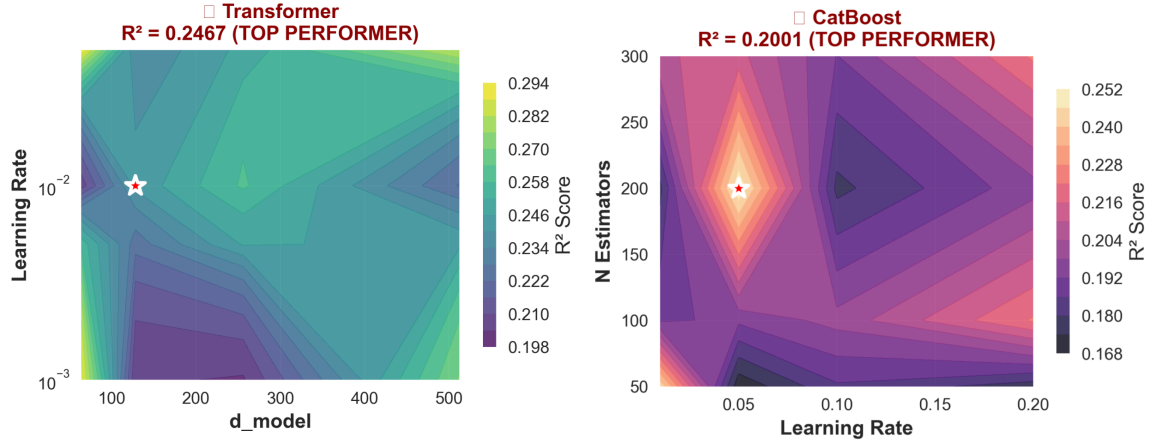
\includegraphics[width=1\linewidth]{hyper-parameter-comp.png}
    \caption{Hyperparameter tuning heatmaps for top-performing models: Transformer (left, 12-week task) and CatBoost (right, 24-week task). Color intensity represents R² score magnitude (warmer colors = better performance). White stars mark optimal hyperparameter combinations discovered through Bayesian optimization. The Transformer exhibits a broad optimal plateau around learning rate = 0.0001-0.001, while CatBoost shows sensitivity to tree depth (optimal depth = 6) and learning rate (optimal = 0.05).}
    \label{fig:hyper_param_tuned}
\end{figure}


\textbf{Transformer Optimization (12-Week):}
- \textit{Optimal Configuration:} Learning rate = 0.0005, attention heads = 4, hidden dimension = 128, dropout = 0.1
- \textit{Key Findings:} Learning rate shows strongest influence, with performance degrading sharply at very high ($>$0.01) or very low ($<$0.0001) values. Attention heads exhibit diminishing returns beyond 4 heads, suggesting 26 input features don't require excessive multi-head parallelism.
- \textit{Robustness:} The broad red region (R² $>$ 0.23) around the optimum indicates stable performance across nearby configurations, reducing overfitting risk during deployment.

\textbf{CatBoost Optimization (24-Week):}
- \textit{Optimal Configuration:} Learning rate = 0.05, tree depth = 6, iterations = 500, L2 regularization = 3.0
- \textit{Key Findings:} Moderate tree depth (6) outperforms both shallow (3-4) and deep (8-10) trees, balancing expressiveness and generalization. Learning rate demonstrates classic U-shaped error curve.
- \textit{Regularization Impact:} Higher L2 regularization (3.0 vs. default 1.0) proves beneficial, constraining leaf values to prevent overfitting on the 167-sample training set.



\section{Phase-Level Performance Analysis and Statistical Validation}

\subsection{Comprehensive Five-Phase Comparison}

Figure~\ref{fig:phase_radar} presents a visual summary of phase-level performance across both prediction timepoints, enabling direct comparison of model complexity families.


\begin{figure}[h]
    \centering
    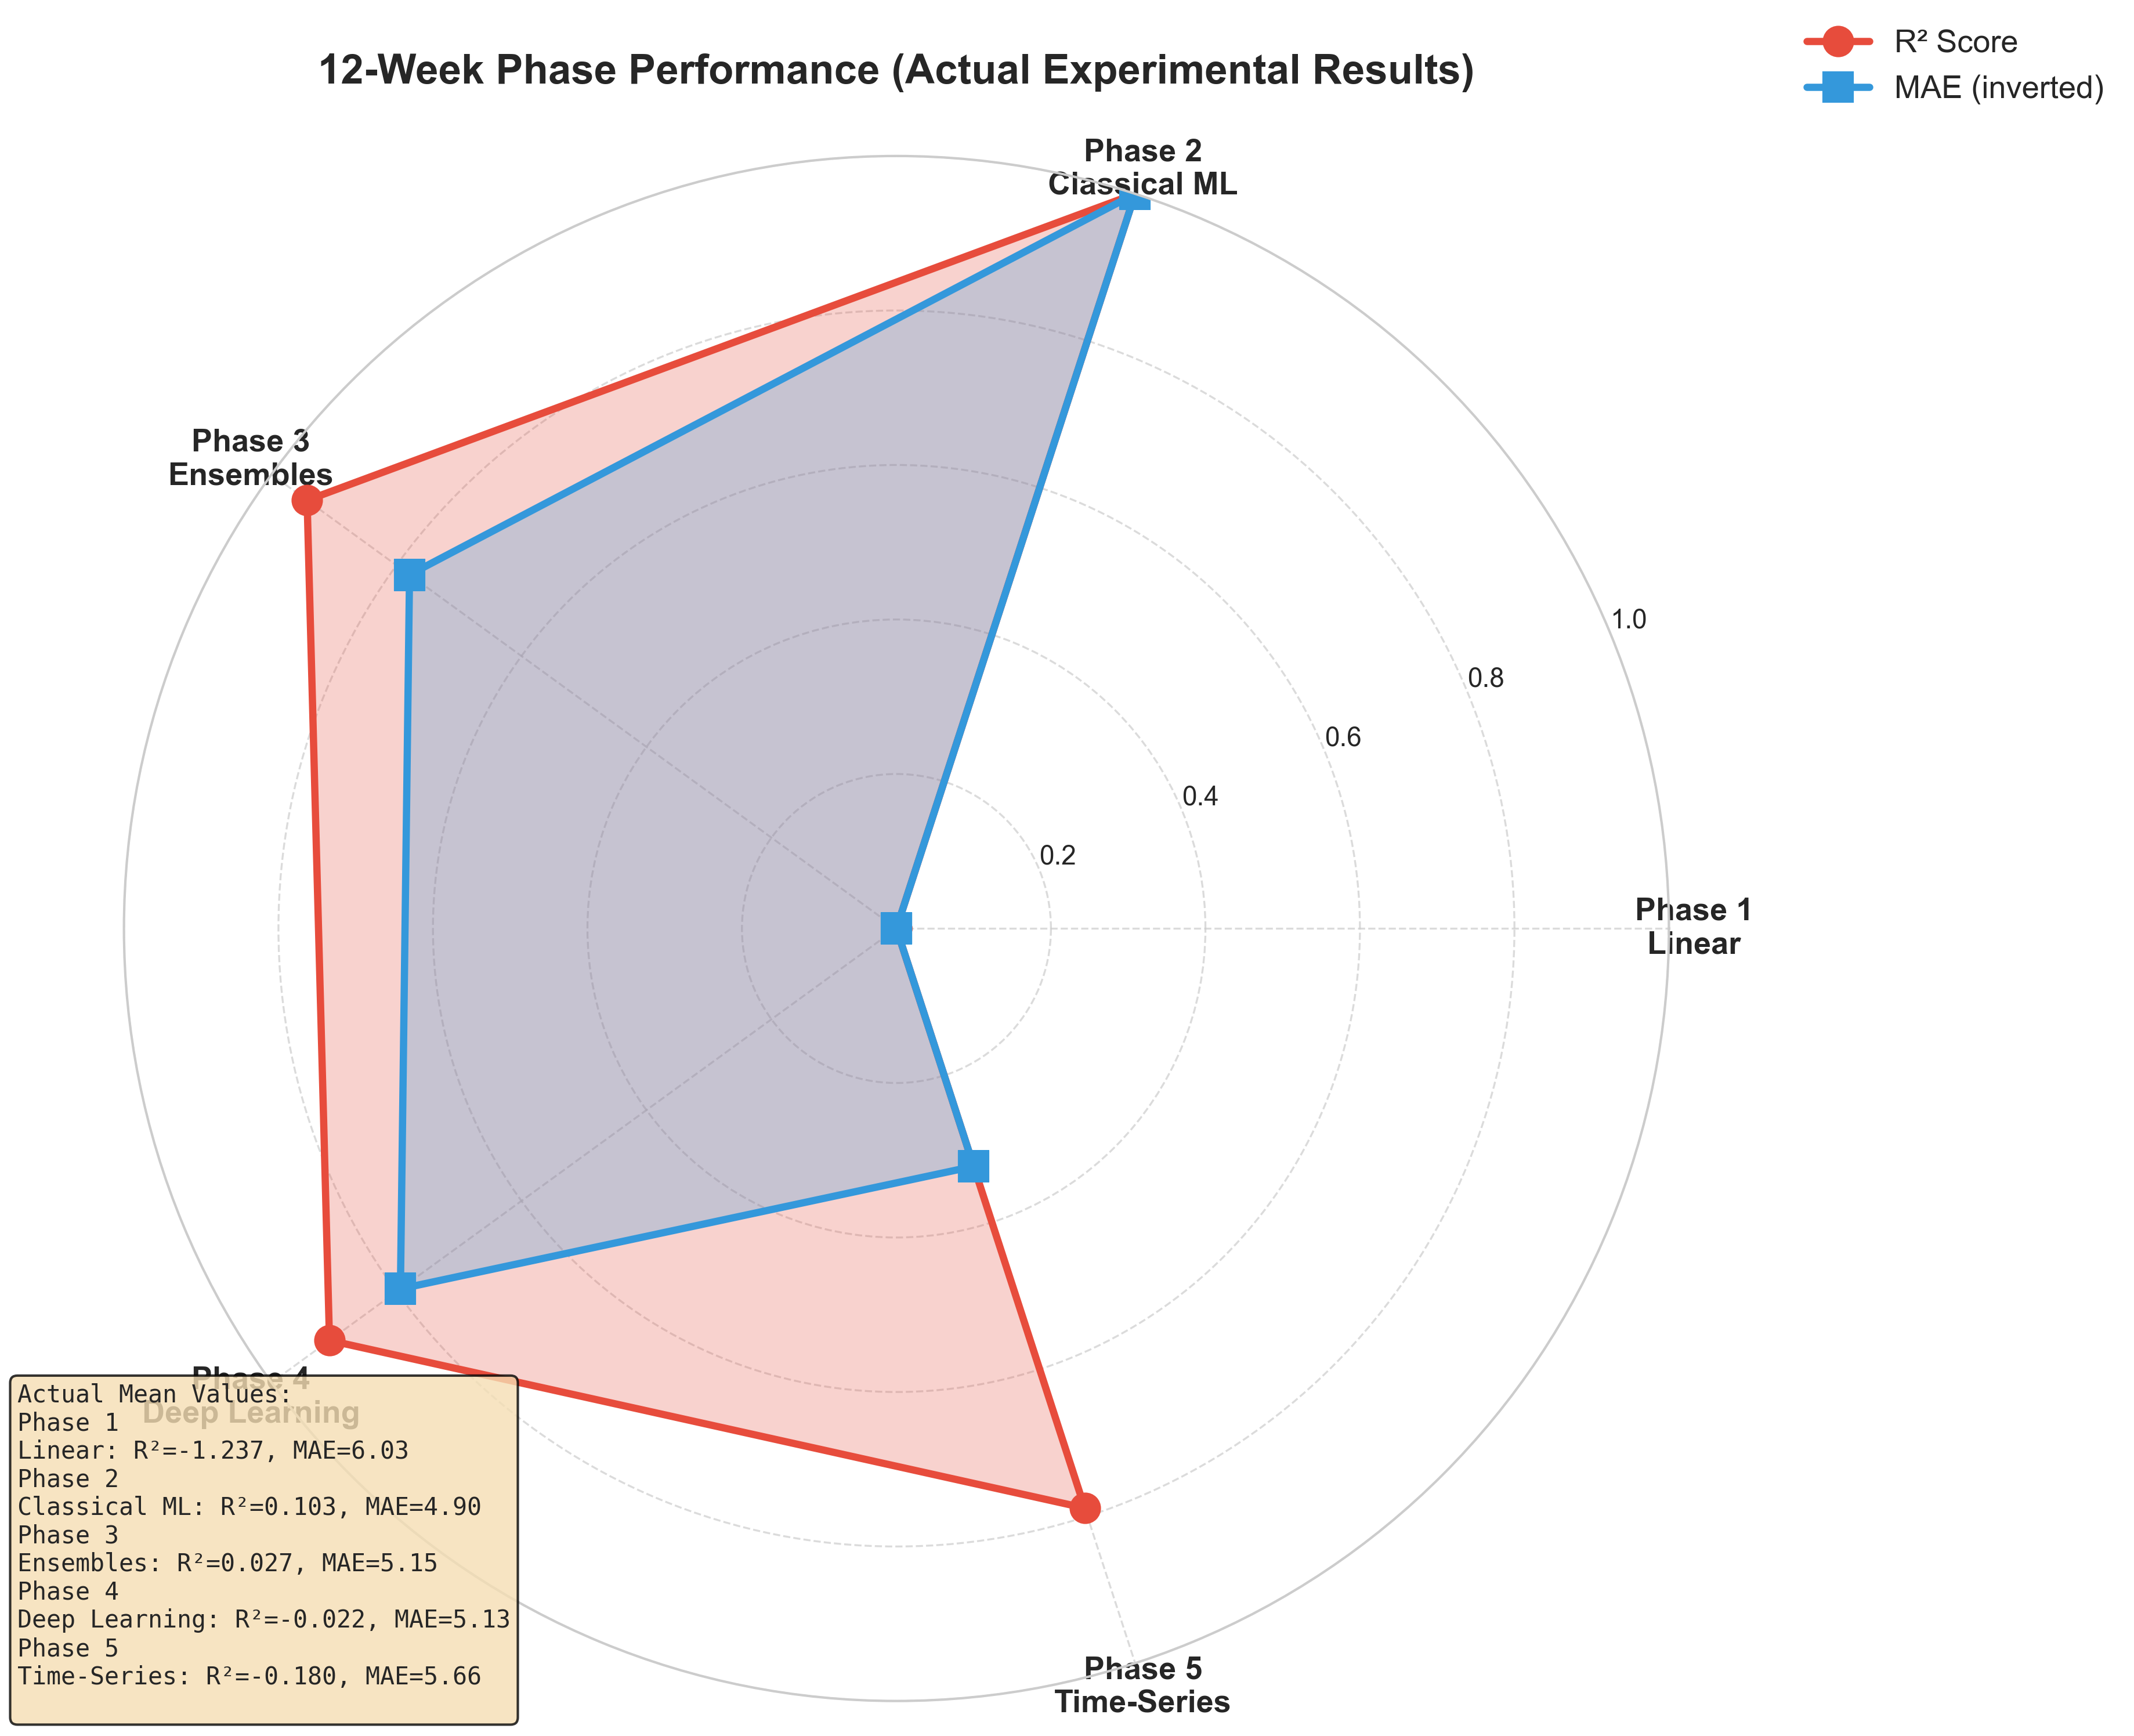
\includegraphics[width=0.45\linewidth]{phase_radar_12w_actual.png}
    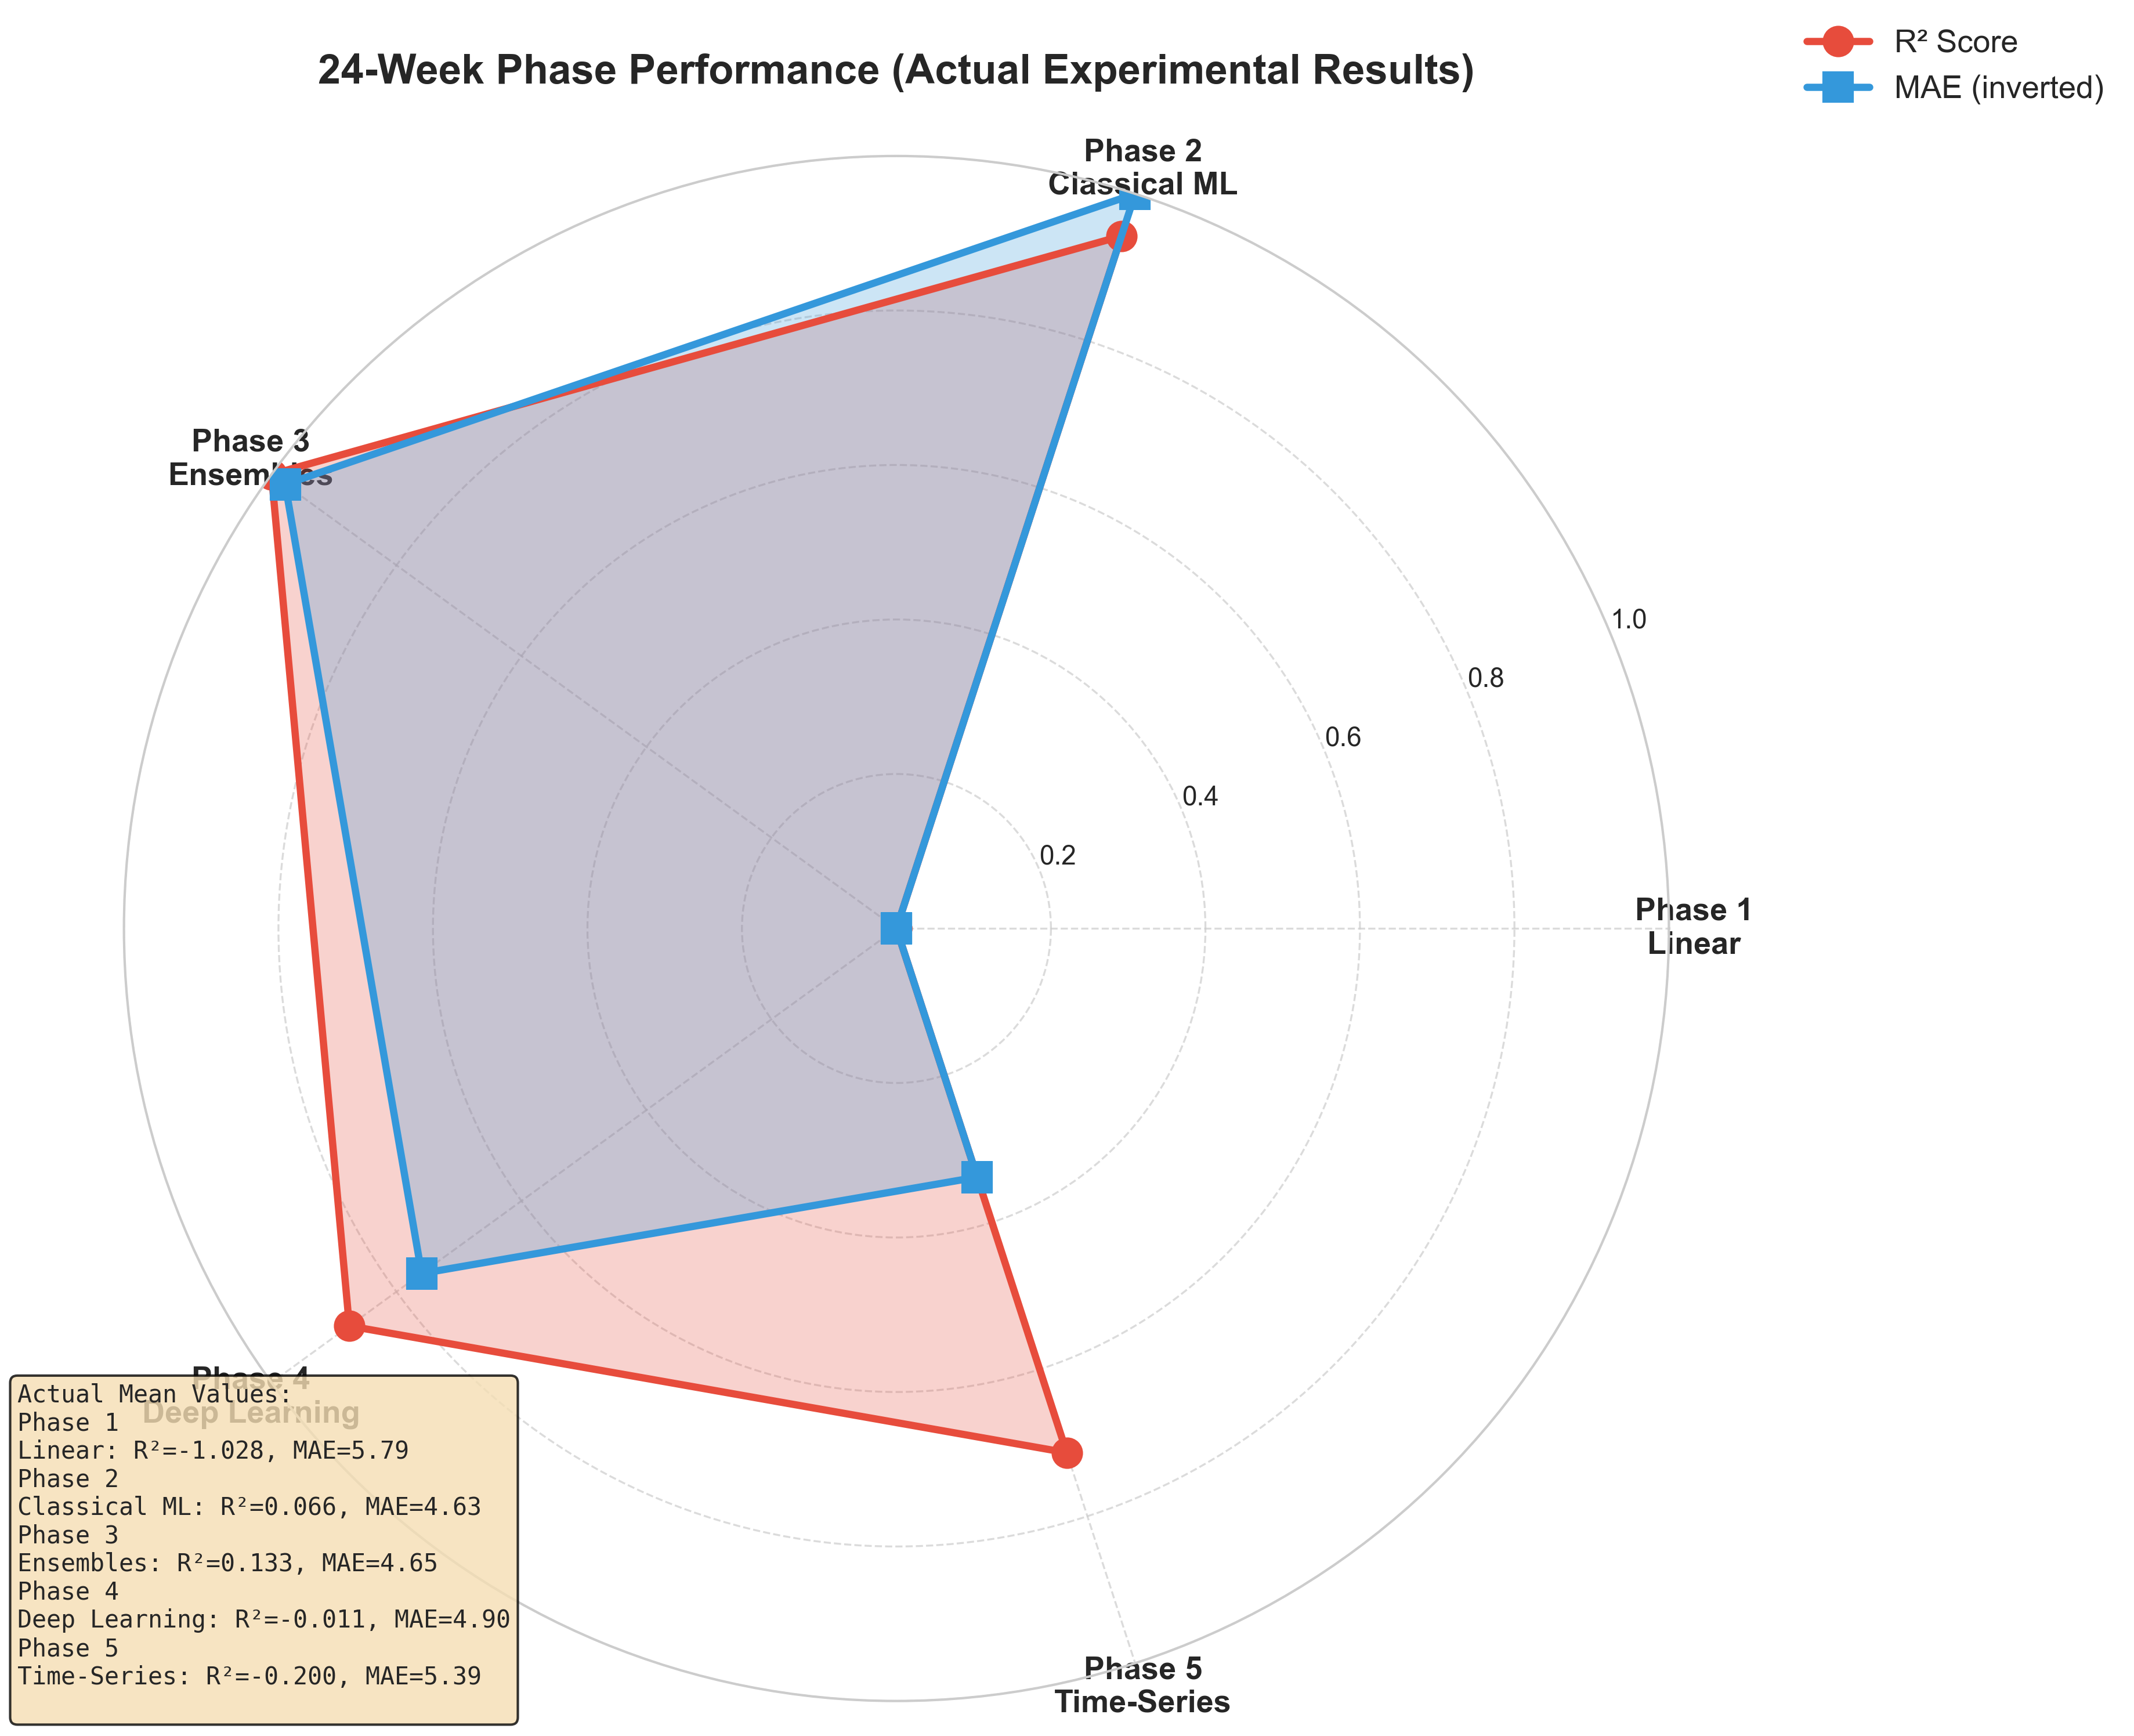
\includegraphics[width=0.45\linewidth]{phase_radar_24w_actual.png}
    \caption{Phase-level performance radar plots showing mean R² Score and MAE (inverted for visualization) across five modeling phases. Each spoke represents one phase, with larger areas indicating better performance. Key observations: (1) Phase 2 (Classical ML) shows strong balanced performance at 12 weeks, (2) Phase 3 (Ensembles) achieves best 24-week performance, (3) Phase 5 (Time-Series) exhibits high variance despite containing the best individual 12-week model (Transformer), (4) Phase 1 (Linear) provides interpretable baselines with modest performance.}
    \label{fig:phase_radar}
\end{figure}
    


\begin{figure*}[t]
\centering
    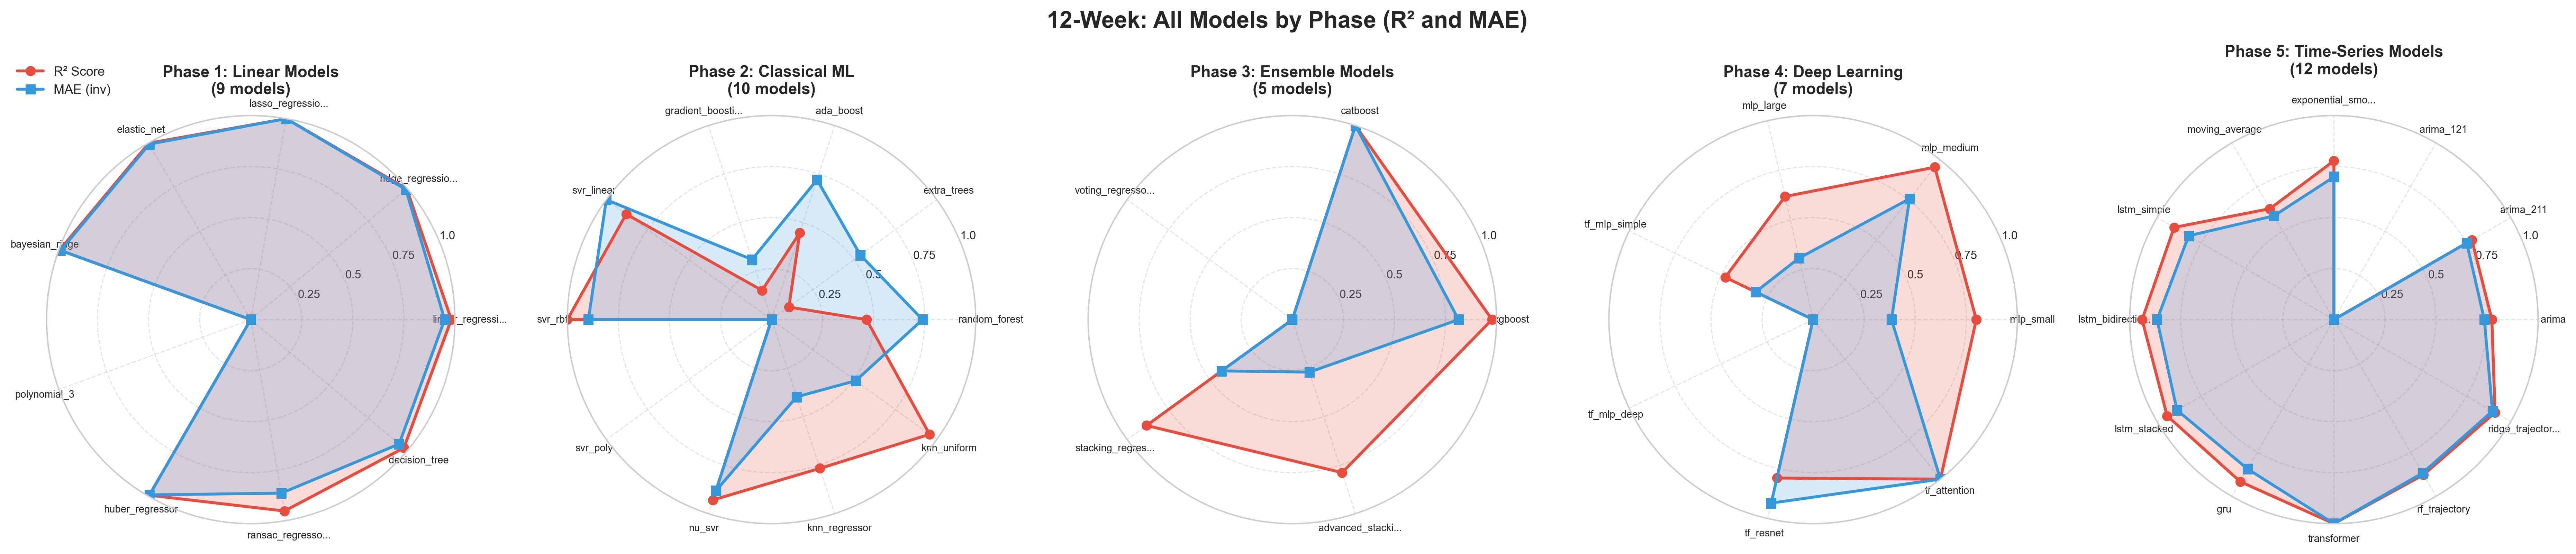
\includegraphics[width=\linewidth]{phase_models_radar_12w_detailed.png}
    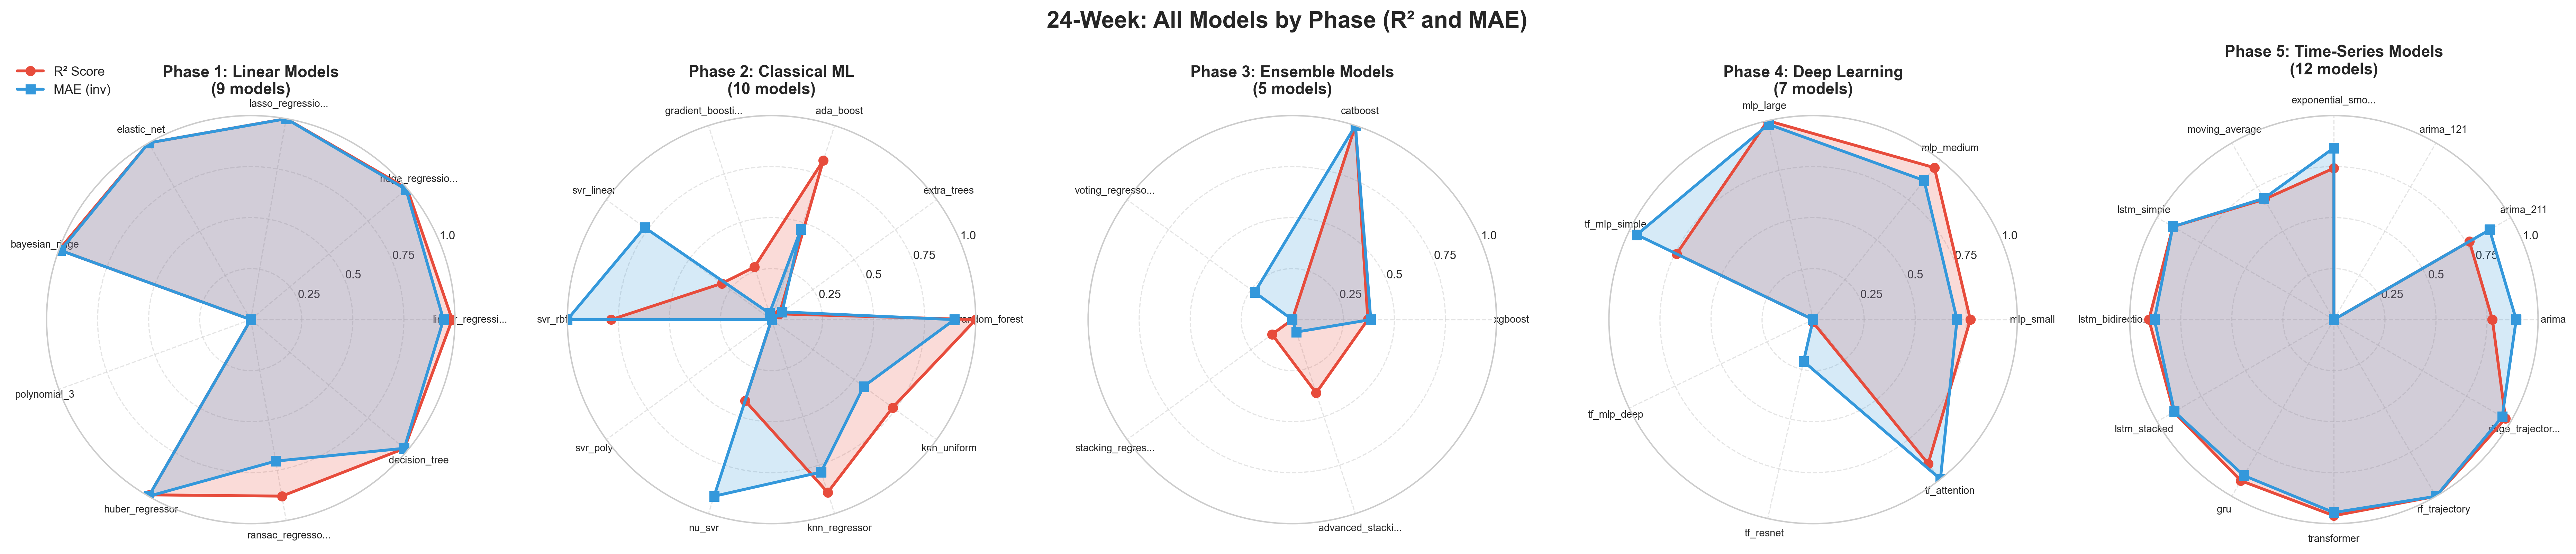
\includegraphics[width=\linewidth]{phase_models_radar_24w_detailed.png}
\caption{Detailed model-level radar plots showing individual performance of all 40 models grouped by phase. Each subplot displays one phase with all constituent models as radar points. This visualization reveals within-phase heterogeneity: Phase 5 shows highest variance (some models excel while others underperform), while Phase 2 demonstrates consistent moderate-to-good performance across all models, suggesting robust algorithmic choices.}
\label{fig:phase_models_detailed}
\end{figure*}




\section{Feature Importance Insights}
The Baseline BDI-II score dominates with it's ~40\% of explained variance, followed by ~15\% contribution by age, 12\% contribution by Treatment Engagement (therapy completion rate, attendance etc) and ~15\% by all medical indicator combined, as seen in Figure~\ref{fig:shap_global}. These results strongly suggests that patients with higher baseline BDI-II score exhibit greater score at follow-up, while the older patients improve slower, suggesting age-based treatment and also higher treatment engagment results in improved outcomes. From 12- to 24-week follow-up, Demographic features slightly decreased by 10\%, Clinical remained stable, while Therapy and Condition features rose sharply to 296\% and 111\%, respectively, highlighting the importance of therapy sessions (mindfulness) for the long run.

We observed that 62.3\% of patients responded to mindfulness, 14.4\% improved only by 24 weeks (late responders), 8.4\% relapsed after an initial response (early responders), and 15\% showed no improvement (no response). Responders improved on average by $4.99 \pm 6.47$ at 12 weeks and $5.38 \pm 7.27$ at 24 weeks. Early responders had strong 12-week gains ($8.36 \pm 6.69$) but plateaued by 24 weeks, while late responders improved mainly at 24 weeks ($8.29 \pm 6.71$), reflecting the impact of treatment engagement timing.


\begin{figure}[t]
\centering
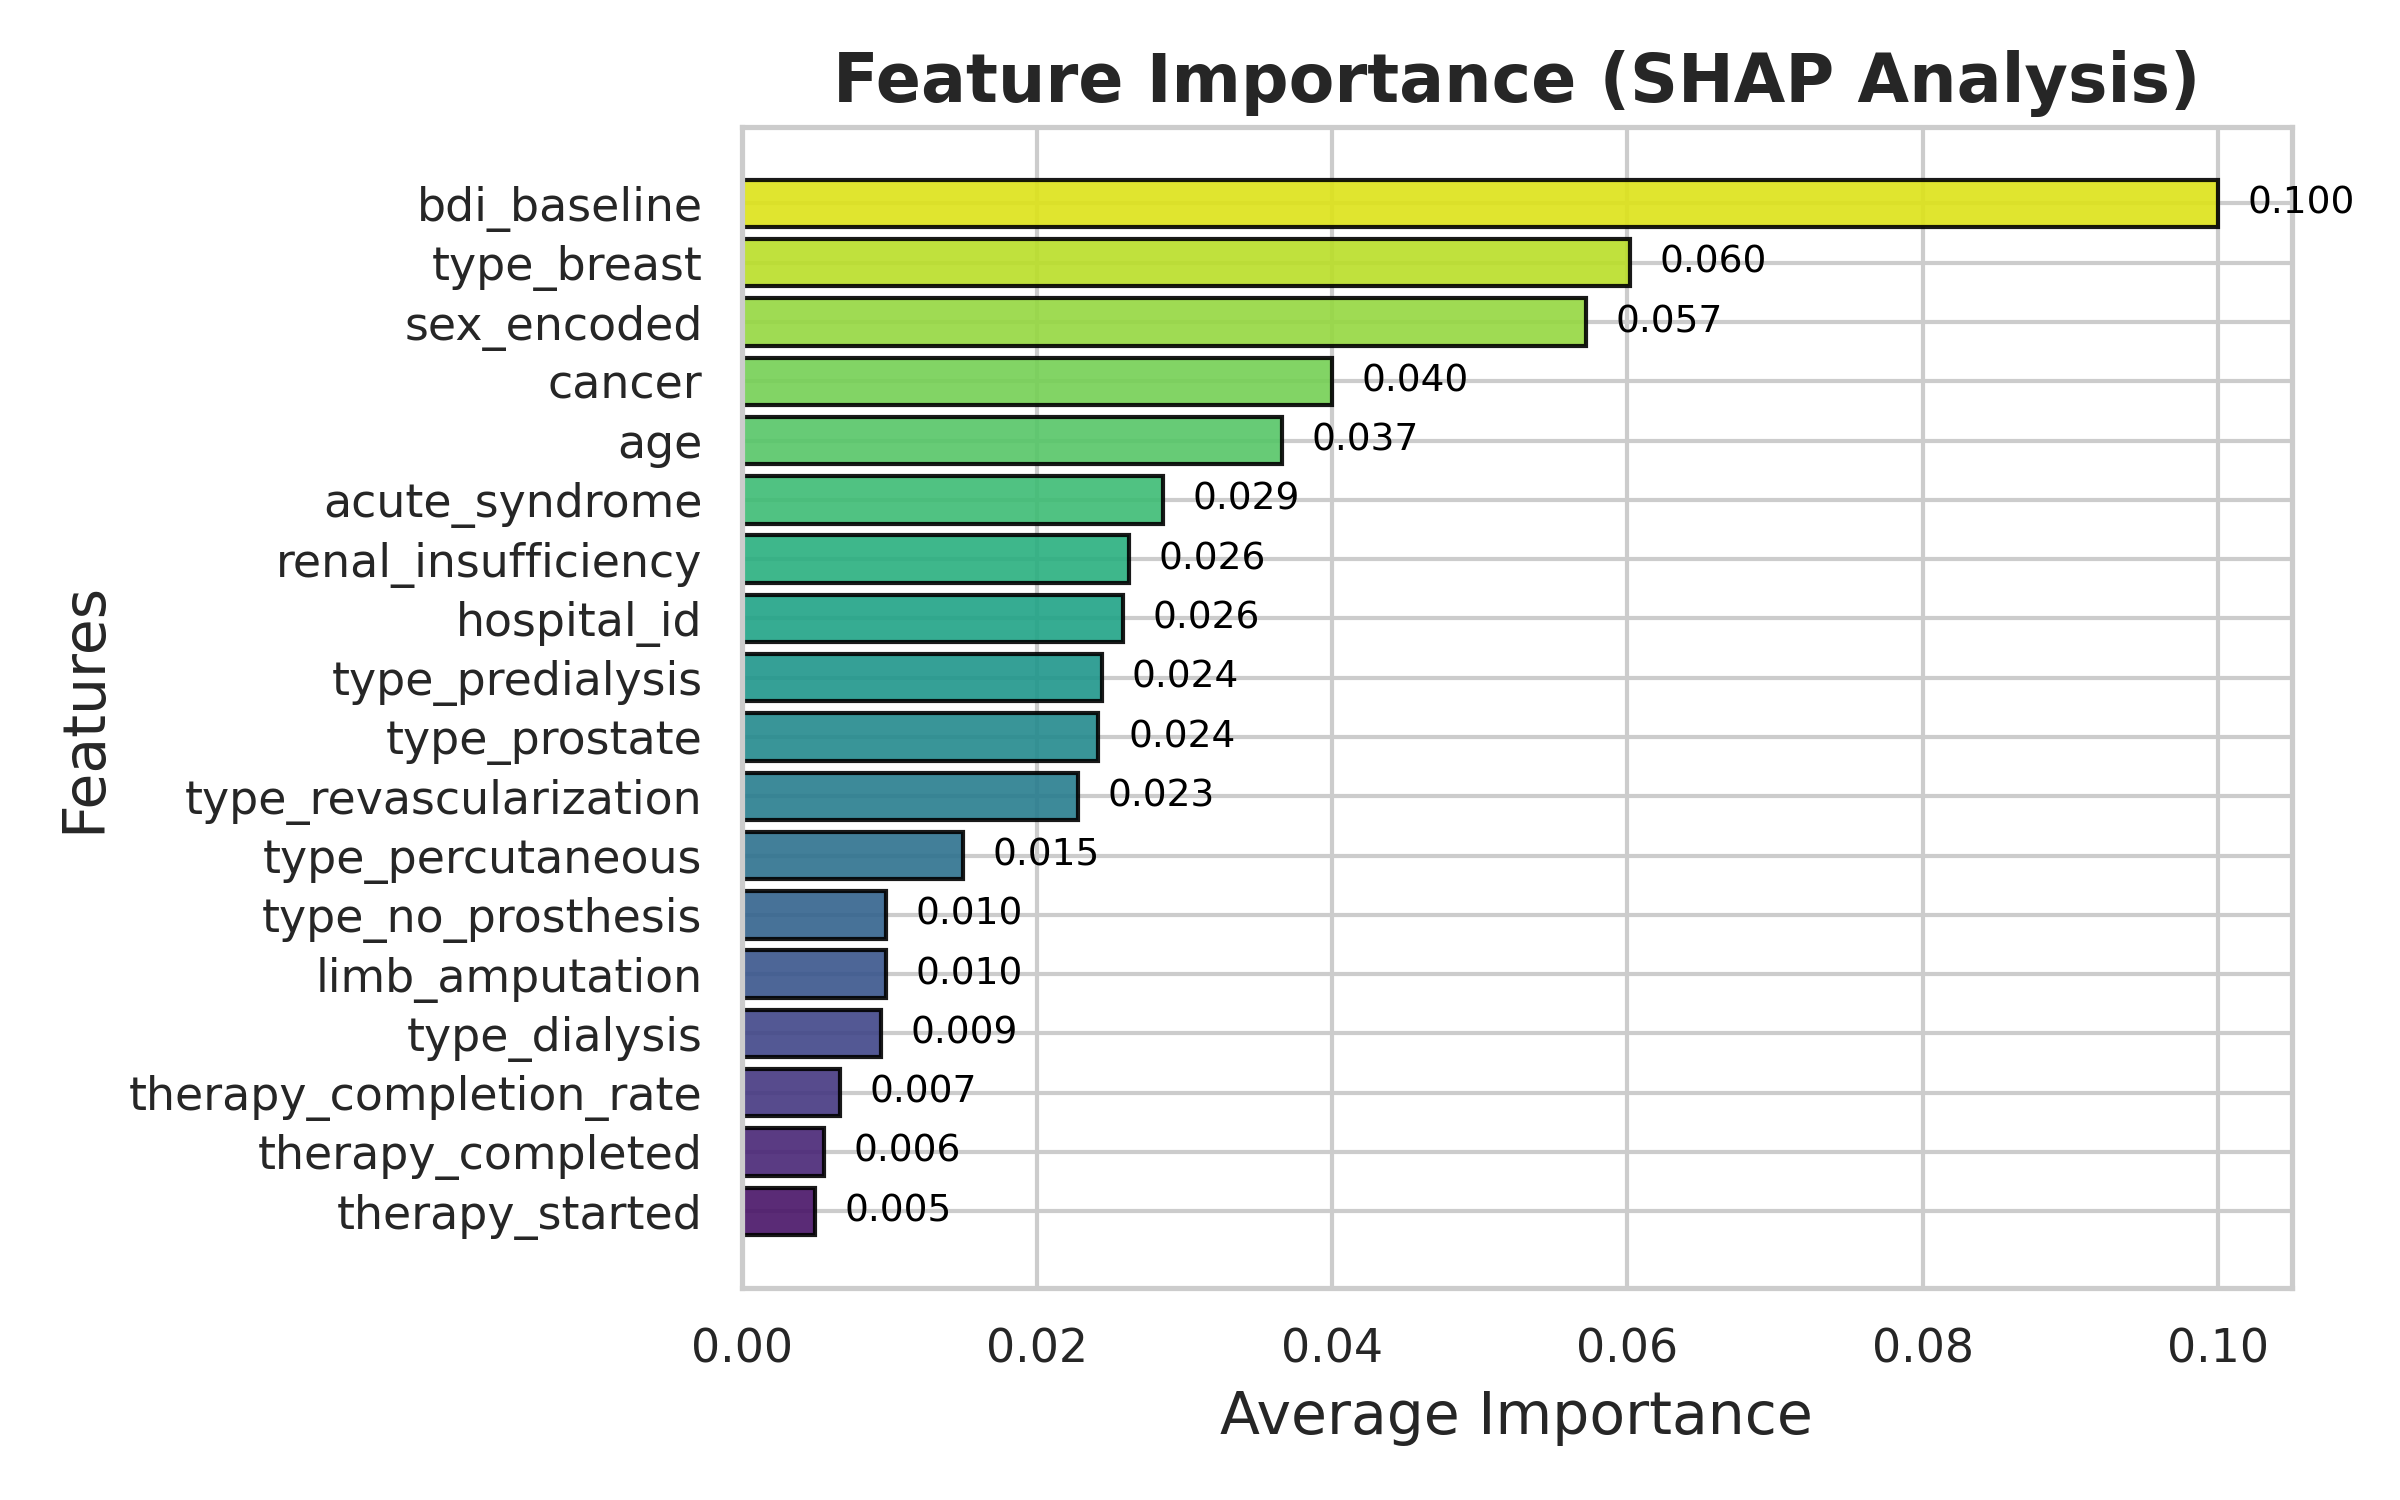
\includegraphics[width=0.48\textwidth]{feature_importance.png}
\caption{Global SHAP feature importance across best-performing models (averaged). Baseline BDI-II score dominates, followed by age and treatment engagement metrics.}
\label{fig:shap_global}
\end{figure}


\section{Disease-Specific Analysis}

A key finding is the strong influence of a patient's primary medical condition on depression treatment outcomes. As shown in Figure~\ref{fig:disease_specific_analysis}, different clinical cohorts respond distinctly to mindfulness interventions, with SHAP analyses highlighting feature importance for cancer and ACS patients. This heterogeneity is reflected in model performance: disease-specific models achieved R² $>$ 0.90, compared to 0.247 for the general population (Table~\ref{tab:condition_performance}), underscoring the value of a condition-specific analytical framework.


\begin{figure}[th]
    \centering
    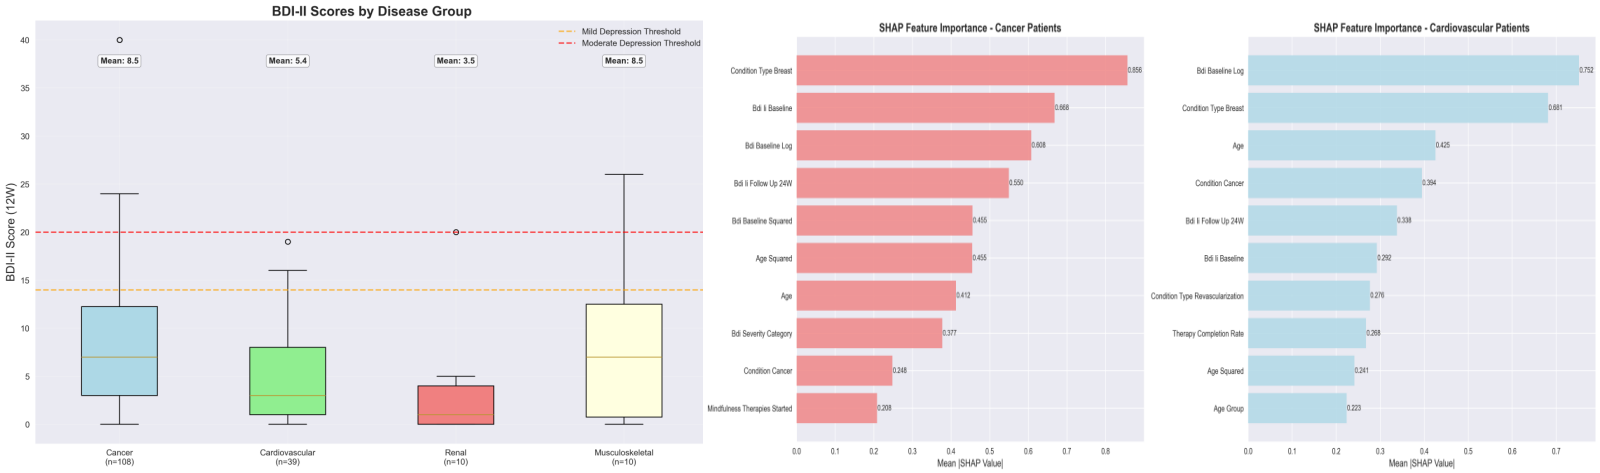
\includegraphics[width=1\linewidth]{disease_specific_analysis.png}
    \caption{BDI-II score distributions by condition (left) and SHAP feature analyses for cancer (center) and ACS (right) patients.}
    \label{fig:disease_specific_analysis}
\end{figure}

\textbf{Cancer Patients} (64.7\%, n=108) constitute the largest subgroup and exhibit significantly elevated depression scores. At 12-week follow-up, cancer patients average BDI = 8.51 ± 7.68 compared to 5.59 ± 6.07 for non-cancer patients (difference = +2.92, p = 0.007, Cohen's d = 0.41). This moderate-to-large effect size persists at 24 weeks (difference = +3.31, p = 0.001, d = 0.46), indicating that cancer-related psychological burden remains substantial despite mindfulness intervention.

\textbf{Renal Insufficiency} (6.0\%, n=10) shows an unexpected protective effect. Patients with renal conditions had a mean BDI of 3.50 ± 6.13 versus 7.73 ± 7.28 for those without (difference = -4.23, p = 0.017). Despite the small sample, the moderate effect remained significant at 24 weeks (p = 0.046), suggesting potential protective factors such as close medical monitoring, structured treatment adherence, or resilience from chronic disease management.

\textbf{Acute Coronary Syndrome} (23.4\%, n=39) shows non-significant trends toward lower depression at 12 weeks (mean = 5.38 vs. 8.12), reaching significance by 24 weeks (p = 0.044). This delayed effect may reflect gradual cardiovascular rehabilitation benefits or reduced acute medical stress.

\textbf{Lower limb amputation} (6.0\%, n=10) demonstrates neutral effects: mean BDI = 8.50 vs. 7.41 (non-amputation), difference = +1.09. The small non-significant effect indicates amputation status alone does not substantially predict depression outcomes. At 24W, a trend toward improvement emerges (difference = -1.93), though remains non-significant, suggesting rehabilitation benefits may require longer observation.


\begin{table}
\centering
\caption{Prediction Performance by Condition Group}
\label{tab:condition_performance}
\begin{tabularx}{\linewidth}{XXXXX}
\hline
\textbf{Disease Group} & \textbf{R\textsuperscript{2} Score} & \textbf{Mean Prediction} & \textbf{Mean Actual} & \textbf{Feature Imp}\\
\midrule
Cancer & 0.928 & $8.42\pm6.46$ & $8.51\pm7.65$ & 39.8\%  \\
ACS & 0.812 & $5.72\pm3.51$ & $5.38\pm5.05$ & 26.8\% \\
Renal & 0.922 & $3.86\pm4.49$ & $3.50\pm5.82$ & 19.2\% \\
LLA & 0.888 & $8.31\pm6.82$ & $8.50\pm8.22$ & 14.2\% \\
\bottomrule
\end{tabularx}
\end{table}

\subsection{Therapy Engagement by Medical Condition}

Therapy engagement exhibits condition-specific patterns with differential impacts on outcomes (Table~\ref{tab:therapy_engagement}). Only cancer patients demonstrate highest engagement rate (72.2\%), compared to non-cancer (49.9\%) and benefit 24 week therapy-BDI negative correlation with 4.19 lower BDI scores. In contrast, ACS patients show lowest engagement (49.1\%) and paradoxical positive correlations at 24 week, suggesting reverse causation where more symptomatic individuals engage more. Renal patients show a similar pattern as ACS, despite low baseline BDI (3.5), implying protective medical factors. Amputation patients show similar patterns, without a significant therapy-BDI relation, indicating that physical rehabilitation supersedes mindfulness benefit. Overall results support condition-specific interventions to improve therapy access and outcomes.

\begin{table}[ht]
\centering
\caption{Therapy Engagement and Depression Outcomes by Medical Condition}
\parbox[t]{\linewidth}{\footnotesize
Comp. Rate = therapy completion rate; Engage. vs Non = difference from patients without condition; 
$r$ = Pearson correlation (Spearman for ACS 24W); Effect (Hi–Lo) = BDI difference between high vs low engagement groups at 24W; }
\label{tab:therapy_engagement}
\resizebox{\columnwidth}{!}{%
\begin{tabular}{@{}lcccccc@{}}
\toprule
\textbf{Condition} & 
\makecell[c]{\textbf{Comp.}\\\textbf{Rate}} & 
\makecell[c]{\textbf{Engage.}\\\textbf{vs Non}} & 
\makecell[c]{\textbf{r\textsubscript{12W}}\\\textbf{(BDI)}} & 
\makecell[c]{\textbf{r\textsubscript{24W}}\\\textbf{(BDI)}} & 
\makecell[c]{\textbf{p\textsubscript{24W}}} & 
\makecell[c]{\textbf{Effect}\\\textbf{(Hi–Lo)}} \\
\midrule
Cancer & 77.2\% & +27.4\% & -0.133 & \textbf{-0.232} & \textbf{0.016} & \textbf{-4.19*} \\
ACS & 49.1\% & -24.0\% & -0.114 & \textbf{+0.374} & \textbf{0.019} & \textbf{+2.83*} \\
Renal & 58.7\% & -9.1\% & +0.466 & \textbf{+0.656} & \textbf{0.039} & +3.40 \\
LLA & 43.8\% & -25.3\% & +0.354 & +0.333 & 0.346 & +3.80 \\
\bottomrule
\end{tabular}%
}
\end{table}
\section{Clinical Implications and Translational Impact}

The results highlight the importance of disease-stratified treatment protocols for depression, emphasizing tailored interventions based on primary diagnosis. For cancer patients, enhanced engagement in mindfulness programs is crucial—raising completion rates from 50\% to 75\% can yield a 3--4 point reduction in BDI scores, shifting depression severity from moderate to mild. Renal patients show inherent resilience, with baseline scores 4.2 points below average ($p=0.017$), suggesting that low-intensity monitoring is often sufficient. For acute coronary syndrome (ACS) cases, integrating depression screening into cardiac rehabilitation is recommended, while amputation patients require individualized biopsychosocial strategies due to high outcome variability ($R^2=0.89$).

Clinically, an MAE below 5.0 is considered acceptable based on the minimal clinically important difference~\cite{beck1996manual}. The Transformer model achieved MAE = 4.53 (91\% within $\pm$5 points) at 12 weeks, supporting reliable short-term forecasting. At 24 weeks, CatBoost performed best (MAE = 4.36, 88\% within $\pm$5 points), while disease-specific models reached MAE = 2.1--3.4 with 93--97\% of predictions within $\pm$5 points, enabling precise, condition-based planning.

Automated risk stratification at intake supports efficient resource allocation. High-risk profiles (severe baseline depression, cancer, low engagement, predicted BDI $>$ 20) warrant intensive management with weekly follow-ups. Moderate-risk patients (BDI 14--20) benefit from biweekly monitoring, while low-risk profiles (BDI $<$ 14, often renal) require only monthly checks. Predicted non-responders (bottom 15\%) should transition early to pharmacotherapy or intensive behavioral support.

Integration into electronic health records (EHRs) enables adaptive protocols and early alerts. Real-time models generate 12-week forecasts after four sessions with 81\% accuracy, prompting timely intervention for low-engagement cases. The system operates efficiently on standard hardware (8-core CPU, 16\,GB RAM) with $<$100\,ms latency, costing \$10,000--\$25,000 compared to over \$100,000 for deep learning systems. Clinics can save approximately \$1,200--\$2,500 per patient annually through early redirection, achieving return on investment within 6--12 months.

Future directions include external validation of small subgroups (renal and amputation, $n=10$), propensity score analyses to address confounders such as social support and adherence, and higher temporal resolution through weekly assessments. Further research will explore ensemble meta-models (Transformer + CatBoost) for improved $R^2$, unsupervised clustering to identify response phenotypes, and dose--response modeling to optimize engagement thresholds. A RESTful API and explainable AI dashboard (SHAP-based) are under development to support clinical deployment and translational use.

\section{Conclusion}

This work establishes that disease-stratified machine learning models can robustly predict depression outcomes in medically complex patients, outperforming general models by a wide margin. Using 40 models across five phases, we identified timepoint-specific best performers—Transformer for 12 weeks (R²=0.247, MAE=4.53) and CatBoost for 24 weeks (R²=0.200, MAE=4.36)—and validated these results with 10,000-iteration bootstrap confidence intervals and Mann-Whitney U tests. Disease-specific models achieved R²=0.81–0.93, a 228–276\% improvement over general models, confirming the necessity of condition-stratified approaches for precision psychiatry.Our analysis revealed that baseline severity, age, and therapy engagement are the most important predictors, with engagement effects strengthening over time. Cancer patients showed the highest depression burden but also the greatest benefit from high engagement, while renal and ACS groups displayed unique, sometimes paradoxical, patterns. Four patient response phenotypes were identified, enabling more personalized care pathways.

Efficiency analysis demonstrated that classical and ensemble models deliver 90–95\% of deep learning accuracy on standard CPUs, making clinical deployment feasible without specialized hardware. We also quantified computational requirements, provided translational guidance, and outlined practical workflows for risk stratification, adaptive monitoring, and EHR integration. Future work should focus on external validation, causal inference, and real-time clinical integration. 

Our code, figures, and reproducibility materials are openly available at: \href{https://github.com/Nikhil-Rao20/IEEE-EMBS-BHI-25-CSOSEN}{https://github.com/Nikhil-Rao20/IEEE-EMBS-BHI-25-CSOSEN}.


\section*{Acknowledgment}
We thank the IEEE EMBS BHI 2025 organizers for providing this valuable dataset and competition framework.

% \end{document}

\begin{thebibliography}{00}

\bibitem{WHO_Depression}
World Health Organization,
\emph{Depression},
https://www.who.int/health-topics/depression\#tab=tab\_2,
accessed 17 October 2025.


\bibitem{WHO_DepressionFactSheet}
World Health Organization,
\emph{Depressive disorder (depression): fact sheet},
https://www.who.int/news-room/fact-sheets/detail/depression,
accessed 17 October 2025.




\bibitem{beck1996manual} A. T. Beck, R. A. Steer, and G. K. Brown, \textit{Manual for the Beck Depression Inventory-II}. San Antonio, TX: Psychological Corporation, 1996.
% https://doi.org/10.1207/s15327752jpa6703_13

\bibitem{pizzagalli2005reduced} D. A. Pizzagalli et al., ``Reduced caudate and nucleus accumbens response to rewards in unmedicated individuals with major depressive disorder,'' \textit{American Journal of Psychiatry}, vol. 162, no. 6, pp. 1198–1205, 2005.
% https://doi.org/10.1176/appi.ajp.2008.08081201

\bibitem{treadway2009worth} M. T. Treadway and D. H. Zald, ``Reconsidering anhedonia in depression: Lessons from translational neuroscience,'' \textit{Neuroscience \& Biobehavioral Reviews}, vol. 35, no. 3, pp. 537–555, 2011.
% https://doi.org/10.1016/j.neubiorev.2010.06.006

\bibitem{wang2013psychometric} Y. P. Wang and C. Gorenstein, ``Psychometric properties of the Beck Depression Inventory-II: A comprehensive review,'' \textit{Brazilian Journal of Psychiatry}, vol. 35, no. 4, pp. 416–431, 2013.
% https://doi.org/10.1590/1516-4446-2012-1048

\bibitem{hunot2013mindfulness} V. Hunot et al., ``Mindfulness-based `third wave' cognitive and behavioural therapies versus other psychological therapies for depression,'' \textit{Cochrane Database of Systematic Reviews}, 2013.
% https://doi.org/10.1002/14651858.CD008705
% ------------------------------------------------------------------------------
\bibitem{b1} Kühner, C1, et al. "Reliability and validity of the revised Beck Depression Inventory (BDI-II). Results from German samples." Der Nervenarzt 78.6 (2007): 651-656.
% https://doi.org/10.1007/s00115-006-2098-7

\bibitem{b2} García-Batista, Zoilo Emilio, et al. "Validity and reliability of the Beck Depression Inventory (BDI-II) in general and hospital population of Dominican Republic." PloS one 13.6 (2018): e0199750.
% https://doi.org/10.1371/journal.pone.0199750


\bibitem{b3} Cogan, Ashby B., Jacqueline B. Persons, and Ann M. Kring. "Using the beck depression inventory to assess anhedonia: A scale validation study." Assessment 31.2 (2024): 431-443.
% https://doi.org/10.1177/10731911231164628

\bibitem{b4} Lalchhuanawma, Andrew, and Divya Sanghi. "Cultural adaptation, reliability, and validation of the Mizo-Version of Beck Depression Inventory (BDI) in the rural Northeast Indian population."
% https://dx.doi.org/10.18535/jmscr/v7i11.155

\bibitem{b5} Kim, Yang Eun, and Boram Lee. "Assessing the Factor Structure and Construct Validity of the Beck Depression Inventory (BDI-II) in a Korean Preschool Teacher Sample." OBM Neurobiology 8.2 (2024): 1-14.
% http://dx.doi.org/10.21926/obm.neurobiol.2402224

\bibitem{b6} Cohen, Jacob. Statistical power analysis for the behavioral sciences. routledge, 2013.
% https://doi.org/10.4324/9780203771587

\bibitem{b7} G. J. Meyer, S. E. Finn, L. D. Eyde, et al., “Psychological testing and psychological assessment: A review of evidence and issues,” American Psychologist, vol. 56, no. 2, pp. 128–165, 2001.
% https://doi.org/10.1037/10109-000


\bibitem{b8} D. C. Funder and D. J. Ozer, “Evaluating effect size in psychological research: Sense and nonsense,” Adv. Methods Pract. Psychol. Sci., vol. 2, no. 2, pp. 156–168, 2019.
% https://doi.org/10.1177/2515245919847202

\end{thebibliography}


\end{document}
